\documentclass[11pt]{article}

\usepackage[utf8]{inputenc}
\usepackage[T1]{fontenc}
\usepackage[margin=2.4cm]{geometry}
\usepackage{graphicx}
\usepackage{booktabs}
\usepackage{amsmath}
\usepackage{siunitx}
\usepackage{xcolor}
\usepackage{float}
\usepackage[font=small,labelfont=bf]{caption}
\usepackage{subcaption}
\usepackage[hidelinks]{hyperref}

\graphicspath{{../results/}{../results/figures/}{../results/paper_assets/}}

\sisetup{detect-weight=true, mode=text}
\newcommand{\best}[1]{\textbf{#1}}

\title{Volumetric Breast Tumor Segmentation in Digital Breast Tomosynthesis
under Low-Resource Conditions:\\ Methodology and Results}
\author{}
\date{}

\begin{document}
\maketitle

%======================================================================
\section{Methodology}
%======================================================================

\subsection{Study Design}
This study investigates the feasibility of deep learning--based volumetric breast
tumor segmentation in digital breast tomosynthesis (DBT) under \emph{low-resource
conditions}, defined as a setting with a limited number of annotated volumetric
datasets comprising both synthetic and clinical DBT cases. The experimental
framework integrates synthetic and clinical data sources under a unified annotation
protocol to enable consistent training and evaluation across heterogeneous datasets.
A comparative framework was implemented to assess three convolutional neural network
architectures --- a baseline 3D U-Net~\cite{cicek2016}, nnU-Net~\cite{isensee2021},
and Attention U-Net~\cite{oktay2018} --- across dataset configurations with varying
lesion sizes and data composition. The study is
structured as a methodological proof-of-concept, focused on feasibility and
comparative model behavior under constrained data conditions rather than on
establishing clinical performance benchmarks. As an additional contribution, a
two-stage \emph{sim-to-real} ensemble was developed to maximize segmentation
performance on the clinical test set (Section~\ref{sec:ensemble}).

\subsection{DBT Datasets: Synthetic and Hybrid Clinical Data}
The synthetic datasets include 30 DBT cases with small lesions
($3$ to $<5$~mm) from the BreasTomo-Synth dataset~\cite{breastomosynth}, and 90 DBT
cases with larger lesions ($>5$ to $7$~mm) from the T-SYNTH dataset~\cite{tsynth}.
Both sources were derived from the FDA-cleared VICTRE knowledge-based simulation
framework~\cite{victre_pipeline,badano2018}, mitigating domain shift between synthetic
configurations. The clinical dataset comprises 20 biopsy-proven malignant DBT cases
from the BCS-DBT benchmark~\cite{bcsdbt}, acquired in real clinical settings.
Synthetic DBT data are used here as a complementary resource for model development
under limited annotation budgets~\cite{alfaro2025}.

Four dataset configurations were defined: (i)~\emph{Large Tumor} (synthetic,
$n=90$); (ii)~\emph{Small Tumor} (synthetic, $n=30$); (iii)~\emph{Mixed-size Tumor}
(synthetic combination, $n=120$); and (iv)~\emph{Hybrid Synthetic--Clinical}, which
combines the mixed-size synthetic data with the clinical DBT cases ($n=140$).

\subsection{Unified Annotation Protocol}
To ensure methodological consistency, all tumor masks were delineated at the voxel
level by a single expert with 20 years of experience in breast imaging, using
ImageJ/Fiji~\cite{fiji} and a consistent protocol across all datasets. The unified protocol
guarantees comparable labeling criteria across synthetic and clinical data,
enabling a controlled comparison of segmentation performance.

To avoid data leakage, all splits were performed at the study level so that no
slices from the same DBT study were shared across training, validation, and test
sets. For the 3D U-Net and Attention U-Net, the synthetic-only datasets were
partitioned $80\%/10\%/10\%$ (train/val/test). In the Hybrid configuration, $50\%$
of the clinical cases were reserved exclusively for testing, while the remaining
clinical cases were combined with the synthetic data for training and validation
($80\%/20\%$ split of the combined set). This design evaluates generalization to
unseen real-world clinical data. All models were trained on full field-of-view
volumetric inputs without lesion-centered cropping or localization priors.

\subsection{Data Representation and Preprocessing}
Original DBT acquisitions, stored as stacks of axial slices, were converted into
three-dimensional arrays. Each study was represented as a volume of 15 consecutive
slices: a central slice associated with the lesion (the slice with maximum tumor
cross-sectional area in the annotation mask) and seven adjacent slices on each side.
This selection balances anatomical
context with computational feasibility while limiting peripheral reconstruction
artifacts, following a similar strategy reported previously~\cite{shia2024}. For
lesions near the volume edge, the 15-slice window was shifted to maximize tumor
inclusion. The full breast field of view was preserved and no in-plane cropping was
applied, so lesions appear at variable spatial positions and the models must jointly
localize and segment within the anatomical context.

Preprocessing comprised intensity normalization and resizing to a fixed input size
of $512\times256\times15$ in the $(X,Y,Z)$ plane, preserving anatomical structure
and lesion integrity. Predictions were binarized at a threshold of $0.5$ for
voxel-wise evaluation. All preprocessing parameters were fixed across experiments to
ensure reproducibility and comparability. Representative synthetic and clinical
volumes with their tumor masks are shown in Figure~2 of the manuscript.

\subsection{Model Architectures}
Three convolutional neural network architectures, representing complementary modeling
strategies under low-resource conditions, were evaluated for voxel-wise volumetric
tumor segmentation.

The \textbf{nnU-Net} framework~\cite{isensee2021,isensee2018} was included as a
self-configuring approach that automatically adapts preprocessing, network
architecture, and training parameters to the dataset characteristics. Its
three-dimensional encoder--decoder design enables effective handling of volumetric
data and has demonstrated strong performance across a wide range of medical image
segmentation tasks.

The \textbf{Attention U-Net}~\cite{oktay2018} was implemented to investigate the
effect of attention mechanisms on feature representation. By incorporating attention
gates within the skip connections, the model selectively emphasizes spatially relevant
features while suppressing irrelevant activations, which may be beneficial in complex
anatomical contexts.

A baseline \textbf{3D U-Net}~\cite{cicek2016}, trained with binary cross-entropy loss,
was included as a reference model. It follows the canonical encoder--decoder design
adapted to volumetric data and provides a stable, widely used benchmark for
segmentation performance.

\subsection{Training Strategy and Optimization}
All models used a consistent setup with volumetric inputs of fixed depth (15
slices). The baseline 3D U-Net and Attention U-Net were optimized with
AdamW~\cite{loshchilov2017} (learning rate $1\times10^{-3}$, weight decay
$1\times10^{-5}$) under a polynomial decay schedule with a 5-epoch warm-up, for 500
epochs. nnU-Net used its
self-configured optimizer (SGD with Nesterov momentum $0.99$, initial learning rate
$1\times10^{-2}$, polynomial decay) for its default schedule of 1000 epochs (250
iterations/epoch). All models used mixed-precision training~\cite{micikevicius2017}
and a batch size of one due to the volumetric memory footprint.

For every architecture, the \emph{final model was the best-performing checkpoint on
the validation set} (highest Dice), rather than the last epoch, providing an
early-stopping mechanism that controls overfitting and makes the comparison robust
to differences in nominal training budget. The selected checkpoints occurred well
before the maximum budget (epochs 131--414 for nnU-Net; 260--462 for the
full-volume models), indicating that the larger nominal budget conferred no
training-duration advantage. The two regimes are not directly comparable in epoch
terms, as nnU-Net performs 250 patch-based updates per epoch whereas the full-volume
models perform a single update per volume. A fixed random seed ($=42$) was used
throughout, and splitting was performed at the study level. nnU-Net applied
patch-based sampling with foreground oversampling (probability $0.33$); the
full-volume models used full-volume inputs with foreground oversampling
(probability $0.5$). The baseline 3D U-Net used binary cross-entropy loss, while
nnU-Net and Attention U-Net used composite Dice + cross-entropy losses to address
class imbalance.

\subsection{Sim-to-Real Ensemble Fine-Tuning}
\label{sec:ensemble}
To maximize performance on the clinical test set, a two-stage transfer strategy was
combined with a multi-architecture ensemble. \textbf{Stage 1 (warm start):} each
network was initialized from a model trained on the mixed-size synthetic dataset.
\textbf{Stage 2 (fine-tuning on real):} each network was fine-tuned on the 10
clinical development cases with a low learning rate and a Tversky + cross-entropy
loss ($\alpha=0.3$, $\beta=0.7$), prioritizing recall on small, low-contrast
lesions. Model and threshold selection was performed by \emph{5-fold cross-validation
over the 10 development cases}, producing out-of-fold (OOF) predictions used to
choose the ensemble configuration without leakage. The final ensemble averages the
per-voxel tumor probabilities of the three networks (each the mean of its five
folds) with weights selected on the OOF development set (nnU-Net~$=2$, Attention~$=2$,
3D~U-Net~$=3$) and a probability threshold of $0.3$. The ensemble was evaluated once
on the 10 held-out clinical test cases. The 20 clinical patients are disjoint across
development and test, and the synthetic warm-start originates from an independent
source, ensuring a leakage-free protocol.

\subsection{Evaluation Metrics}
Segmentation was evaluated with standard voxel-wise metrics: the Dice coefficient,
Intersection-over-Union (IoU), precision, and recall. All metrics used binarized
predictions (threshold $0.5$ for individual models; $0.3$ for the ensemble, as
selected on the development set), were computed at the volumetric level (per study),
and averaged across each dataset. Experiments were implemented in PyTorch (2.5.1) on
an NVIDIA GeForce RTX 4070~Ti SUPER GPU (16~GB).

%======================================================================
\section{Results}
%======================================================================

\subsection{Quantitative segmentation performance across datasets}
Table~\ref{tab:main} reports the per-study test performance of the three
architectures across the four dataset configurations. Performance is high on the
synthetic Large and Mixed-size datasets, drops on the Small-tumor dataset, and is
lowest on the Hybrid clinical test --- reflecting the domain gap and the difficulty
of low-contrast clinical lesions.

\begin{table}[H]
\centering
\caption{Volumetric test performance (per-study mean) on the four dataset
configurations. Best Dice per configuration in \best{bold}. Clinical generalization
is assessed on the held-out clinical cases of the Hybrid dataset.}
\label{tab:main}
\small
\begin{tabular}{llcccc}
\toprule
Dataset & Model & Dice & IoU & Precision & Recall \\
\midrule
\textbf{Large tumor}
 & nnU-Net            & \best{0.864} & \best{0.766} & 0.883 & 0.861 \\
 & 3D U-Net (baseline)& 0.830 & 0.717 & 0.841 & 0.846 \\
 & Attention U-Net    & 0.778 & 0.643 & 0.766 & 0.812 \\
\addlinespace
\textbf{Small tumor}
 & nnU-Net            & \best{0.560} & \best{0.476} & 0.674 & 0.574 \\
 & 3D U-Net (baseline)& 0.264 & 0.198 & 0.234 & 0.332 \\
 & Attention U-Net    & 0.367 & 0.269 & 0.305 & 0.505 \\
\addlinespace
\textbf{Mixed-size}
 & nnU-Net            & \best{0.841} & \best{0.737} & 0.894 & 0.808 \\
 & 3D U-Net (baseline)& 0.726 & 0.608 & 0.728 & 0.738 \\
 & Attention U-Net    & 0.582 & 0.433 & 0.604 & 0.646 \\
\addlinespace
\textbf{Hybrid (clinical test)}
 & nnU-Net            & 0.353 & 0.279 & 0.586 & 0.365 \\
 & 3D U-Net (baseline)& \best{0.412} & \best{0.298} & 0.542 & 0.473 \\
 & Attention U-Net    & 0.421 & 0.294 & 0.410 & 0.488 \\
\bottomrule
\end{tabular}
\end{table}

\subsection{Training dynamics}
Figure~\ref{fig:curves} shows the training-loss dynamics of the three architectures
on each dataset configuration. All models converge smoothly; the best validation
checkpoint (used for evaluation) is reached well before the nominal budget in every
case. Figure~\ref{fig:trainval} contrasts the training and validation loss of
nnU-Net across the four configurations: the train--validation gap is largest on the
small-tumor and hybrid clinical settings, consistent with their lower test
performance and the limited amount of representative data. The best-validation
checkpoint (dashed line) is selected as the final model, providing an effective
early-stopping criterion. Because per-epoch validation \emph{loss} was logged only by
nnU-Net, Figure~\ref{fig:allarch} reports the validation signal common to all three
architectures --- the validation Dice --- alongside the training loss, for every
architecture and dataset configuration. The validation Dice plateaus early and remains
stable, confirming convergence without late-stage degradation across all models.

\begin{figure}[H]
\centering
\begin{subfigure}{0.49\textwidth}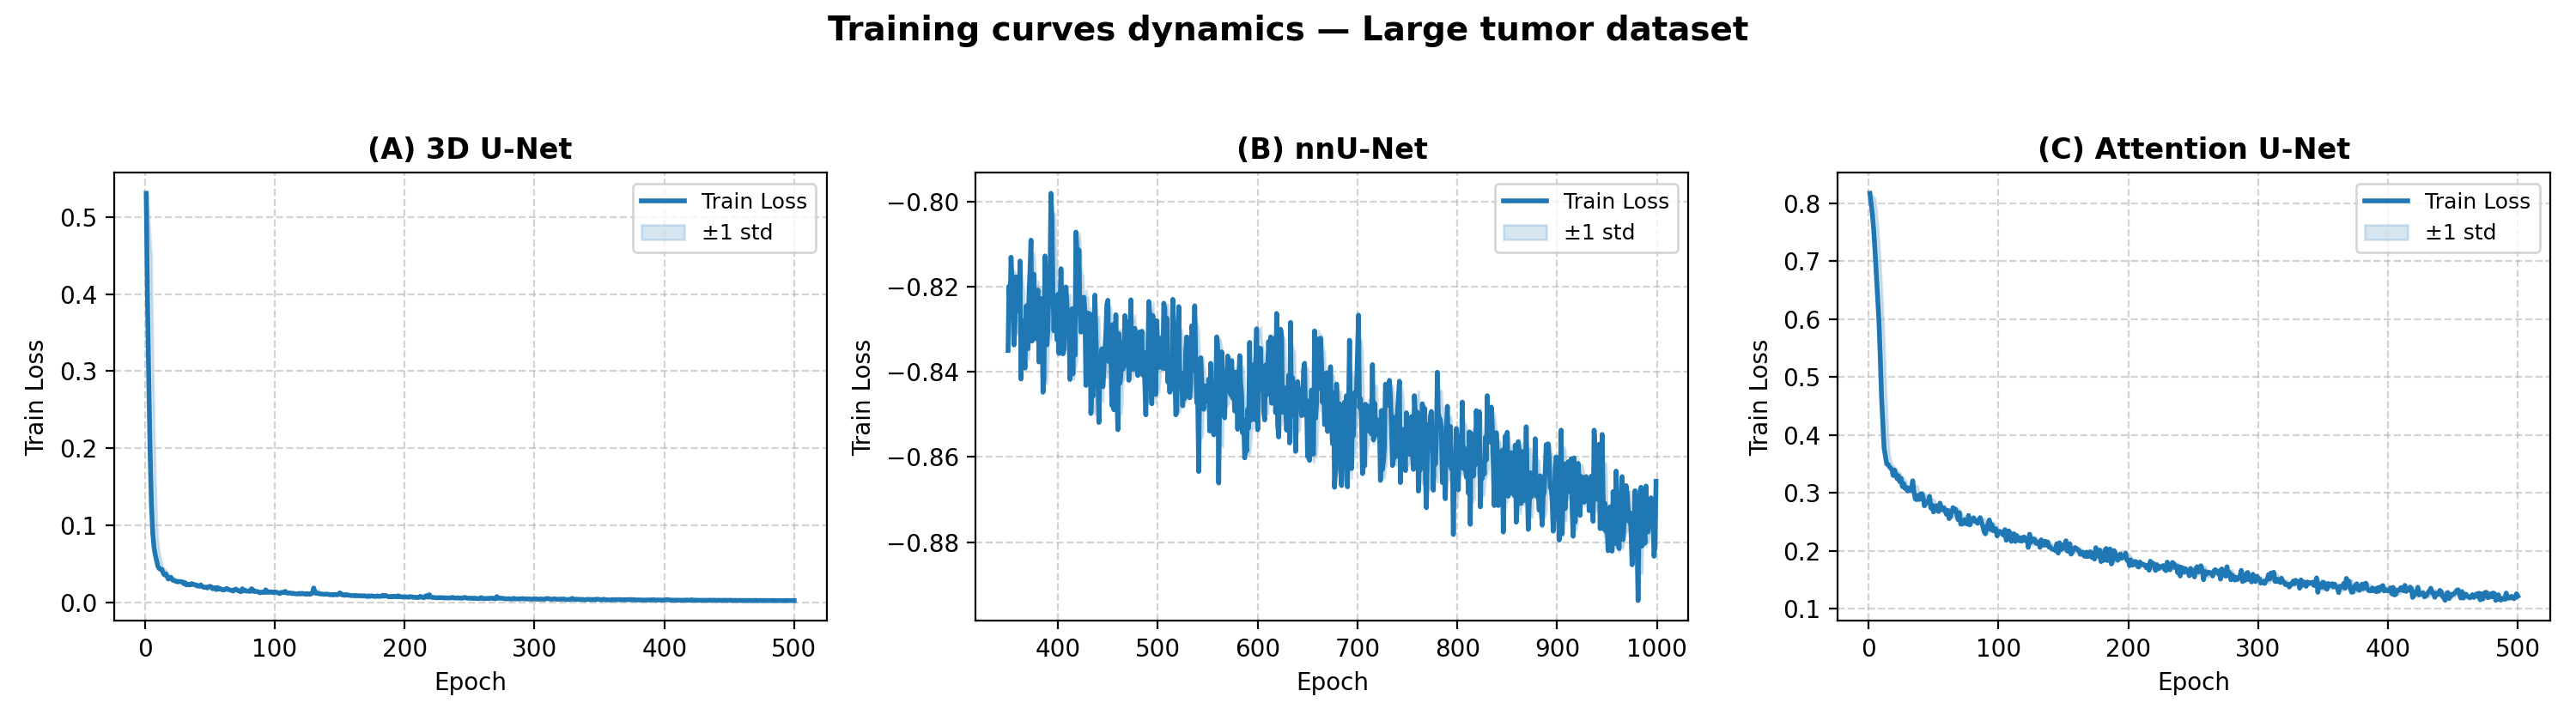
\includegraphics[width=\linewidth]{figures/training_curves_large_tumor.png}\caption{Large tumor}\end{subfigure}\hfill
\begin{subfigure}{0.49\textwidth}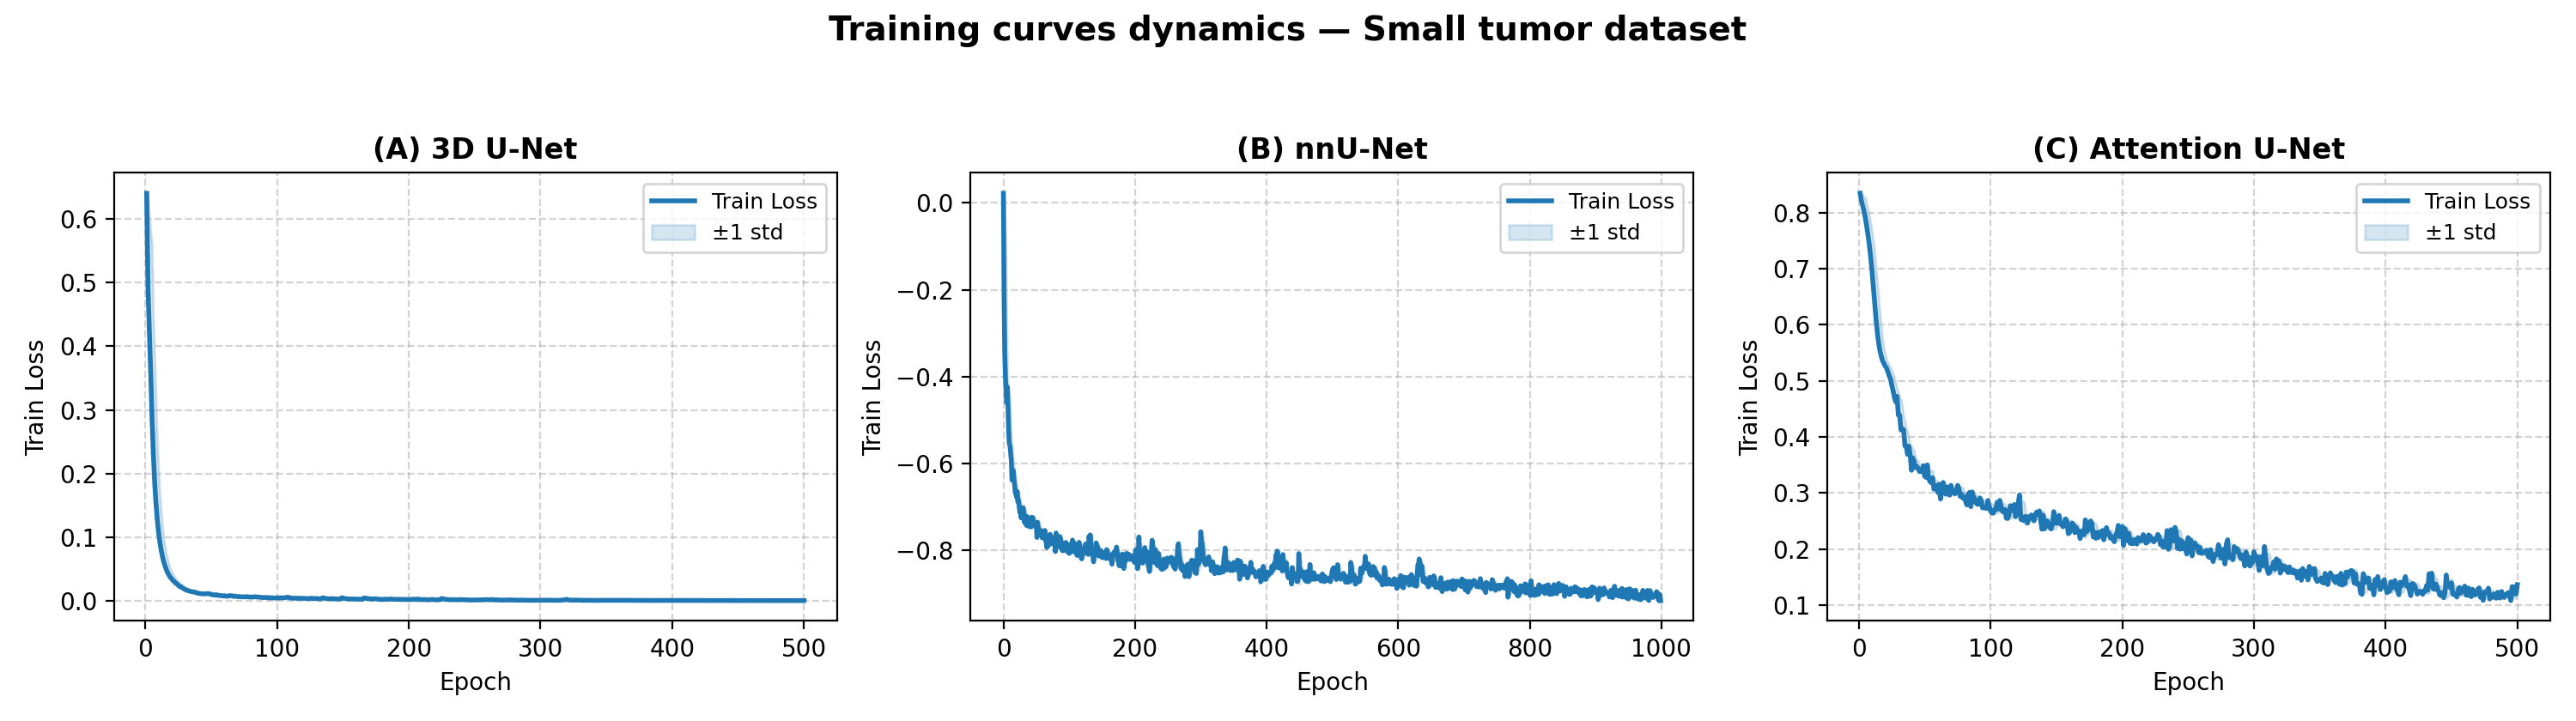
\includegraphics[width=\linewidth]{figures/training_curves_small_tumor.png}\caption{Small tumor}\end{subfigure}

\medskip
\begin{subfigure}{0.49\textwidth}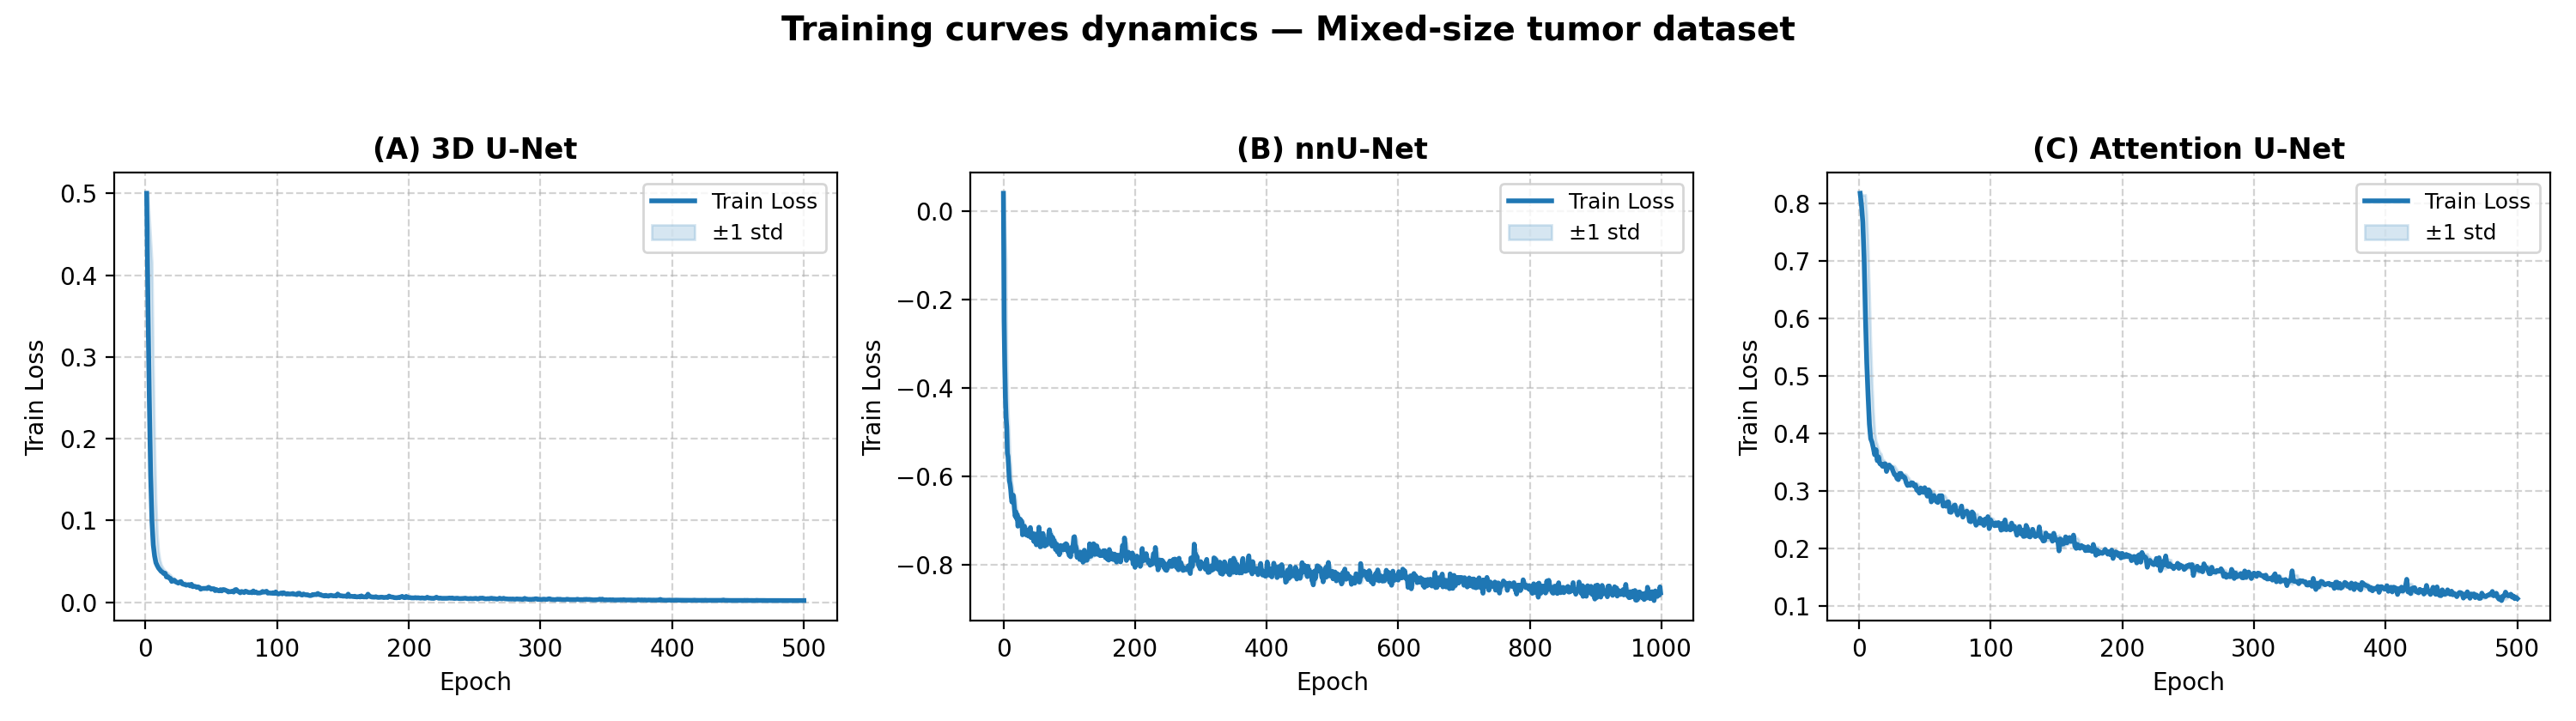
\includegraphics[width=\linewidth]{figures/training_curves_Mixed_Size.png}\caption{Mixed-size}\end{subfigure}\hfill
\begin{subfigure}{0.49\textwidth}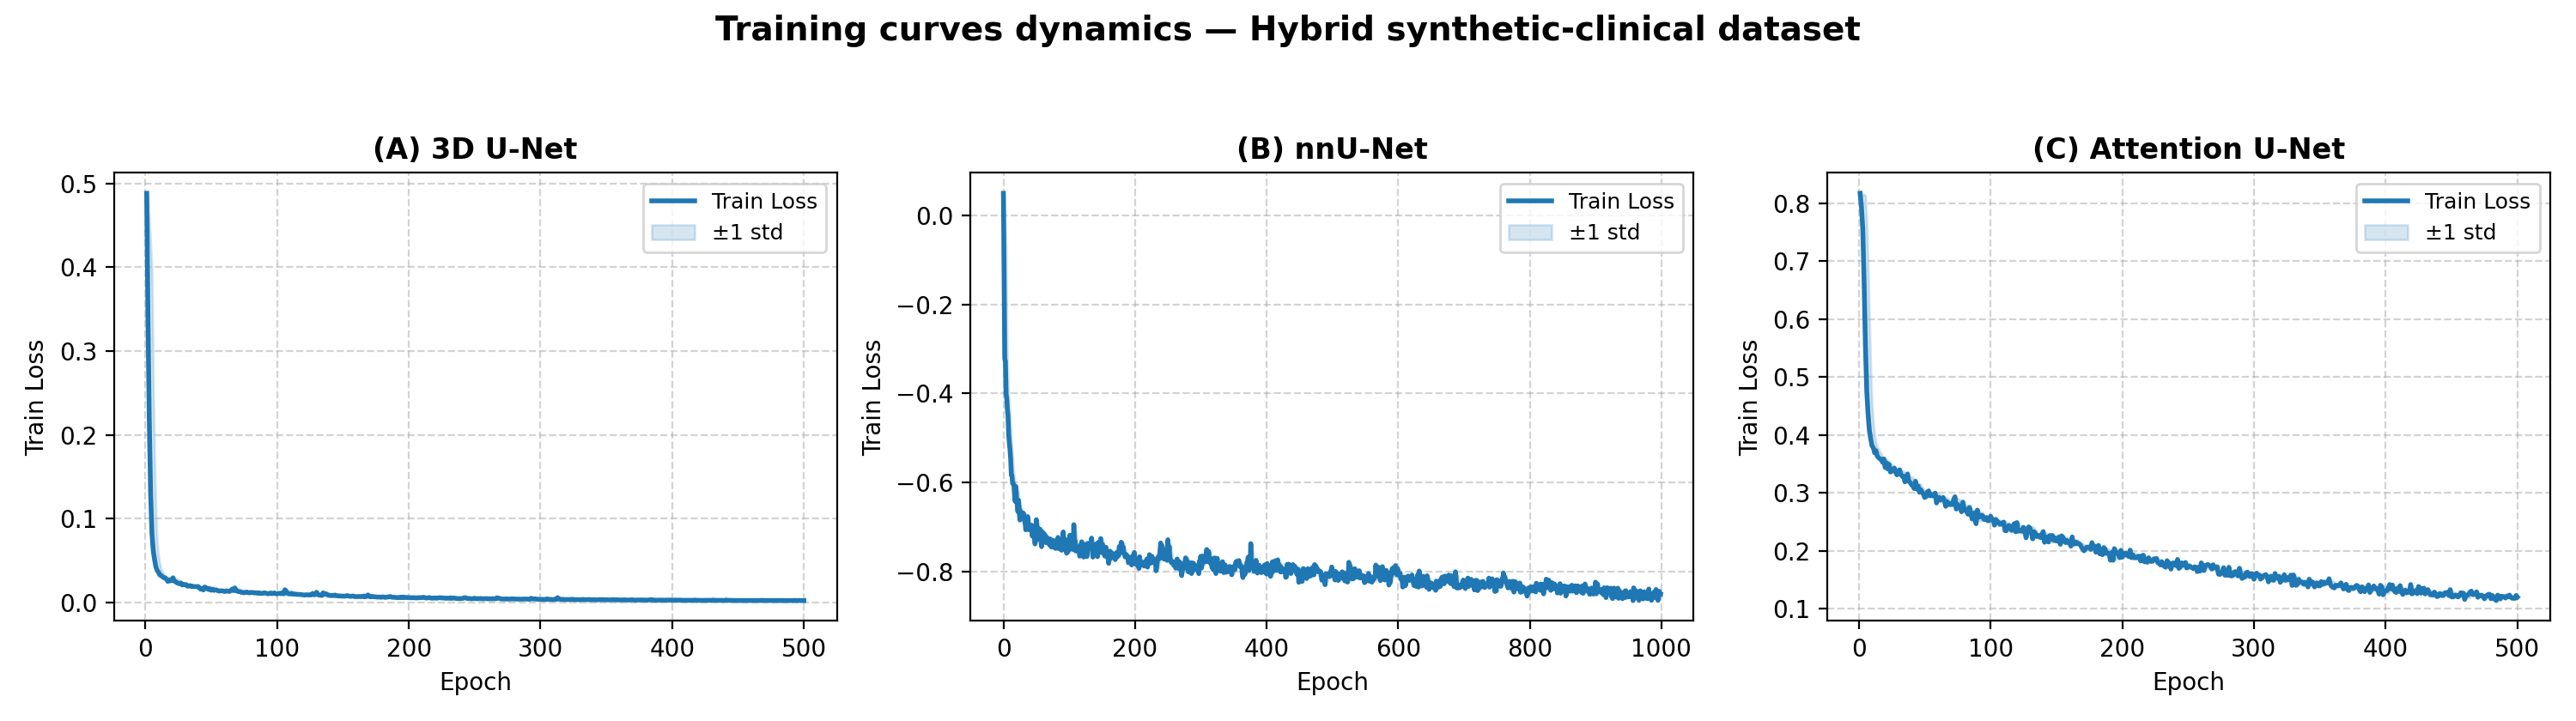
\includegraphics[width=\linewidth]{figures/training_curves_Hybrid.png}\caption{Hybrid synthetic--clinical}\end{subfigure}
\caption{Training-loss curves (mean $\pm$ 1 std) for the 3D U-Net, nnU-Net, and
Attention U-Net across the four dataset configurations.}
\label{fig:curves}
\end{figure}

\begin{figure}[H]
\centering
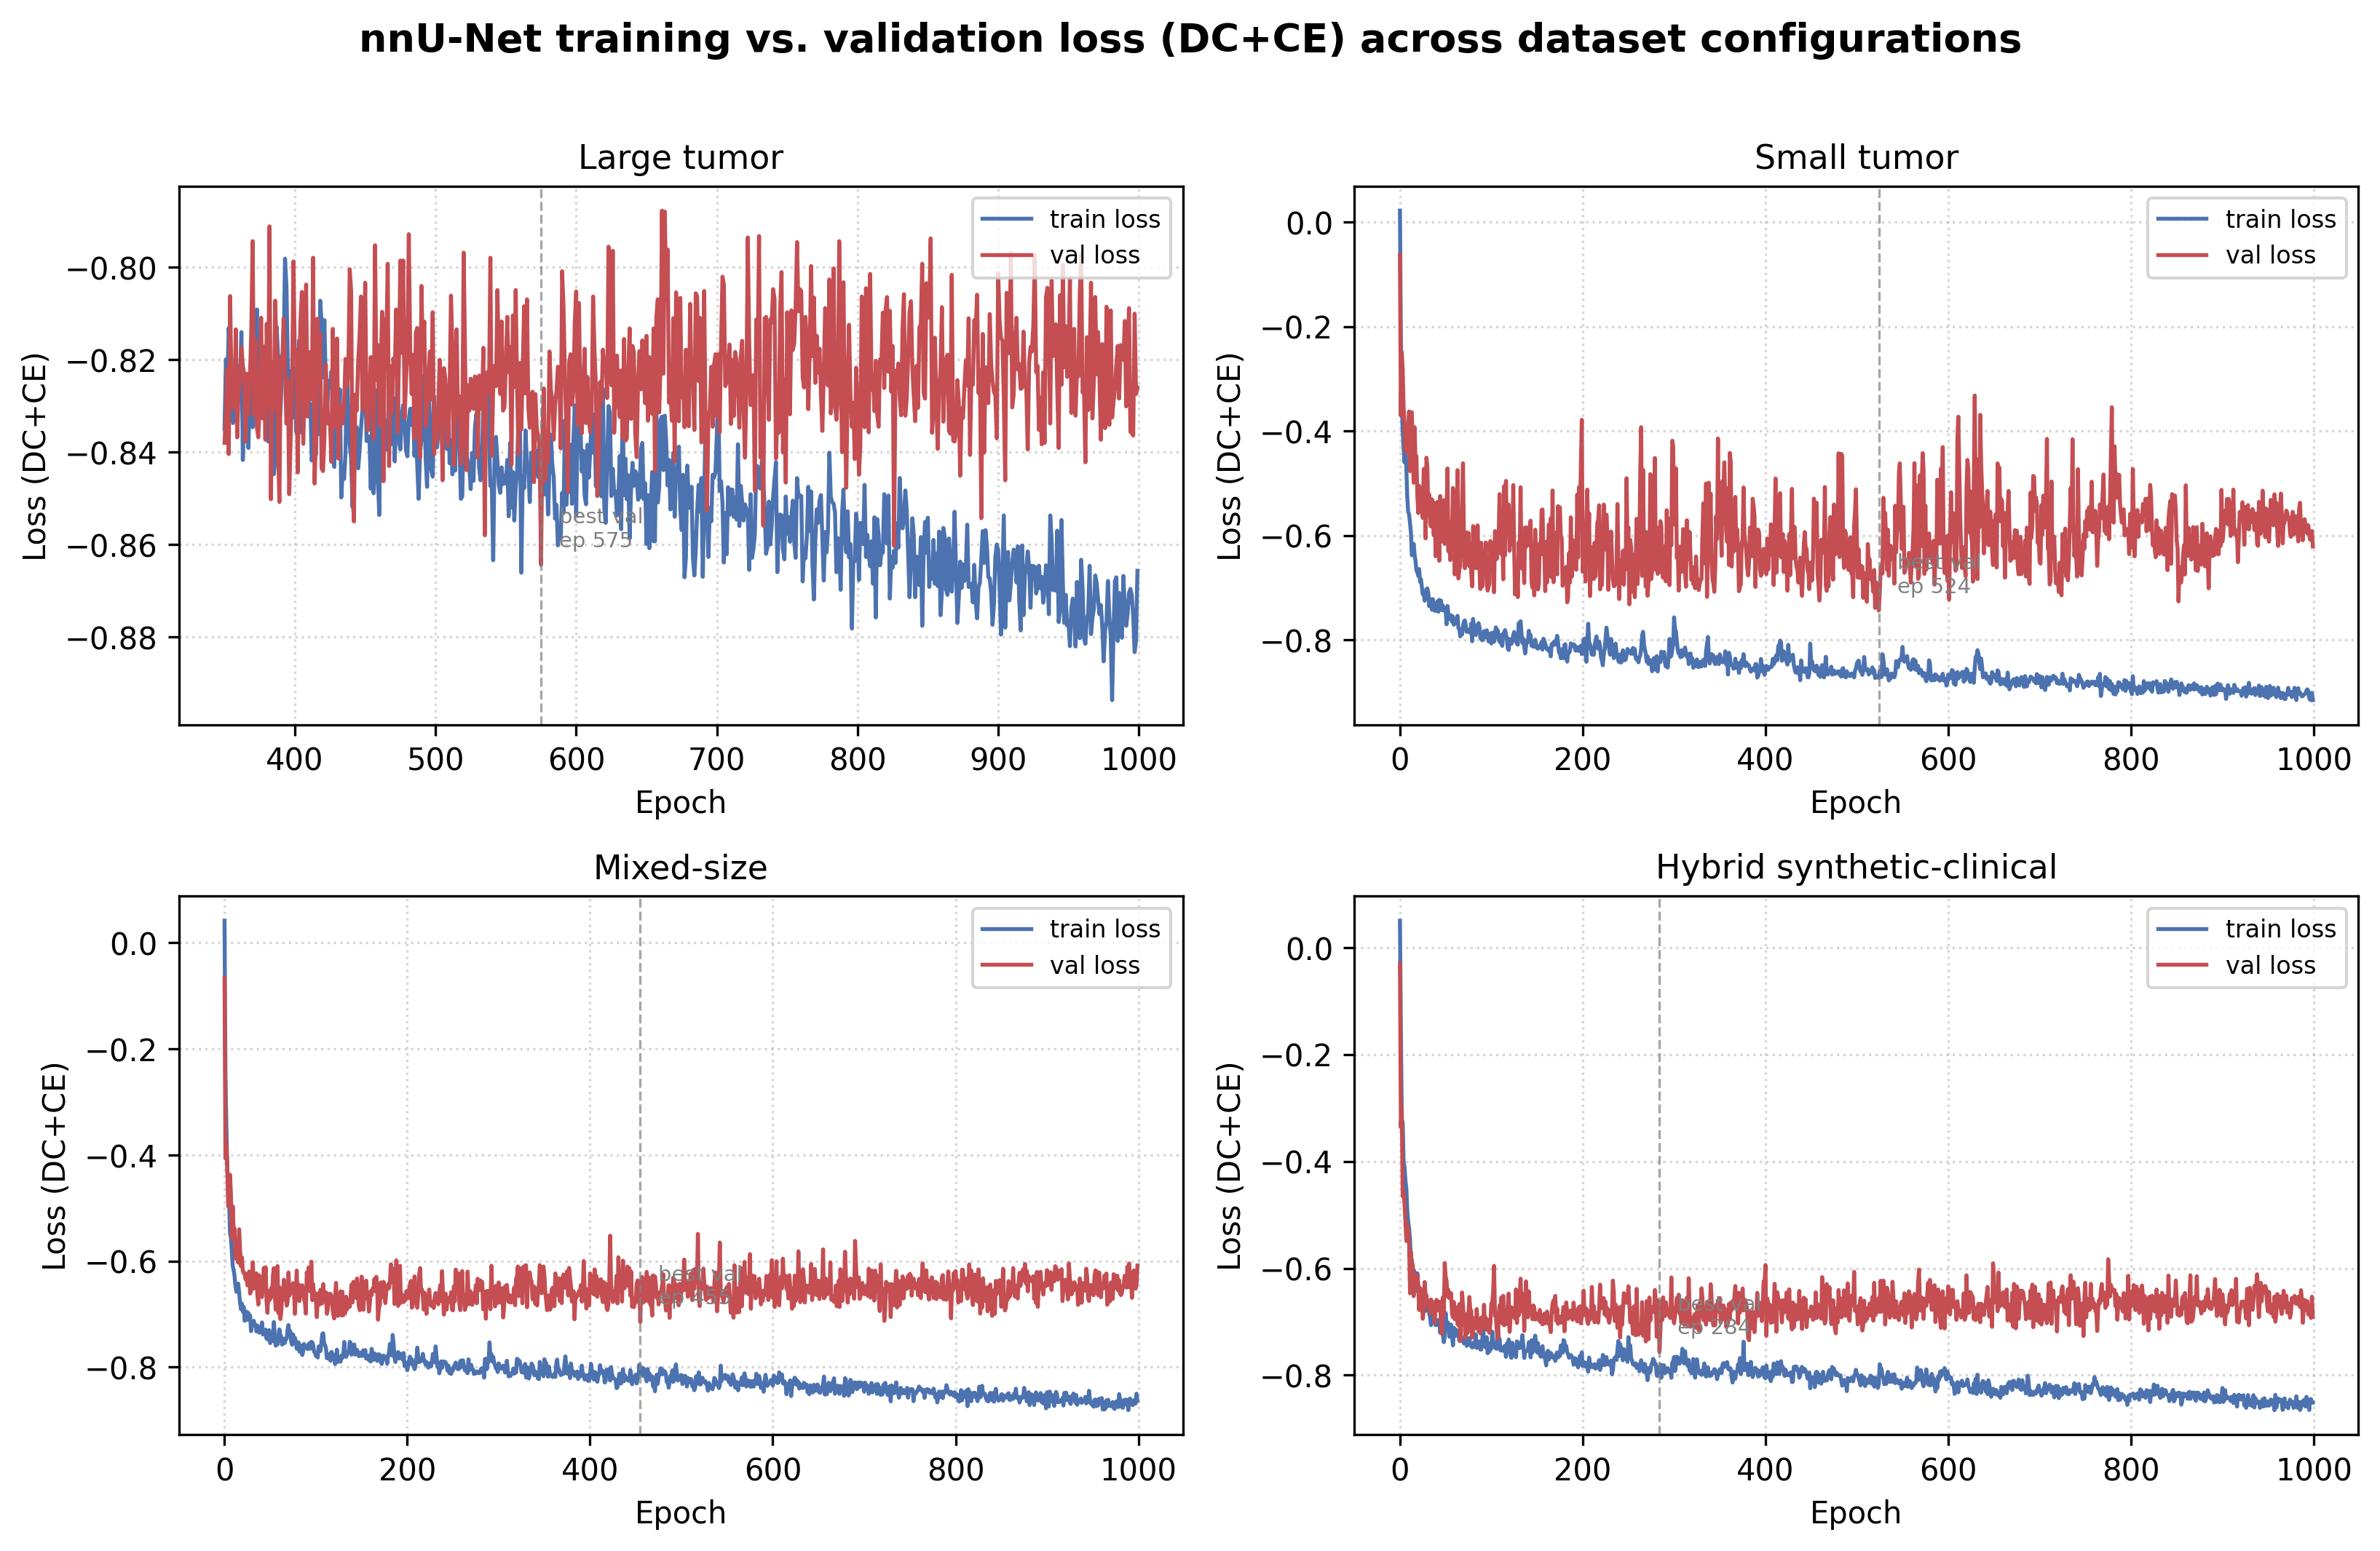
\includegraphics[width=0.92\linewidth]{paper_assets/curves/nnunet_train_val_loss.png}
\caption{nnU-Net training versus validation loss (compound Dice + cross-entropy,
which may be negative) across the four dataset configurations. The dashed line marks
the best-validation epoch used as the final checkpoint. The widening train--validation
gap on the small-tumor and hybrid clinical settings reflects the difficulty of those
regimes. (Validation loss was logged per epoch by nnU-Net; the full-volume models
logged validation overlap metrics instead.)}
\label{fig:trainval}
\end{figure}

\begin{figure}[H]
\centering
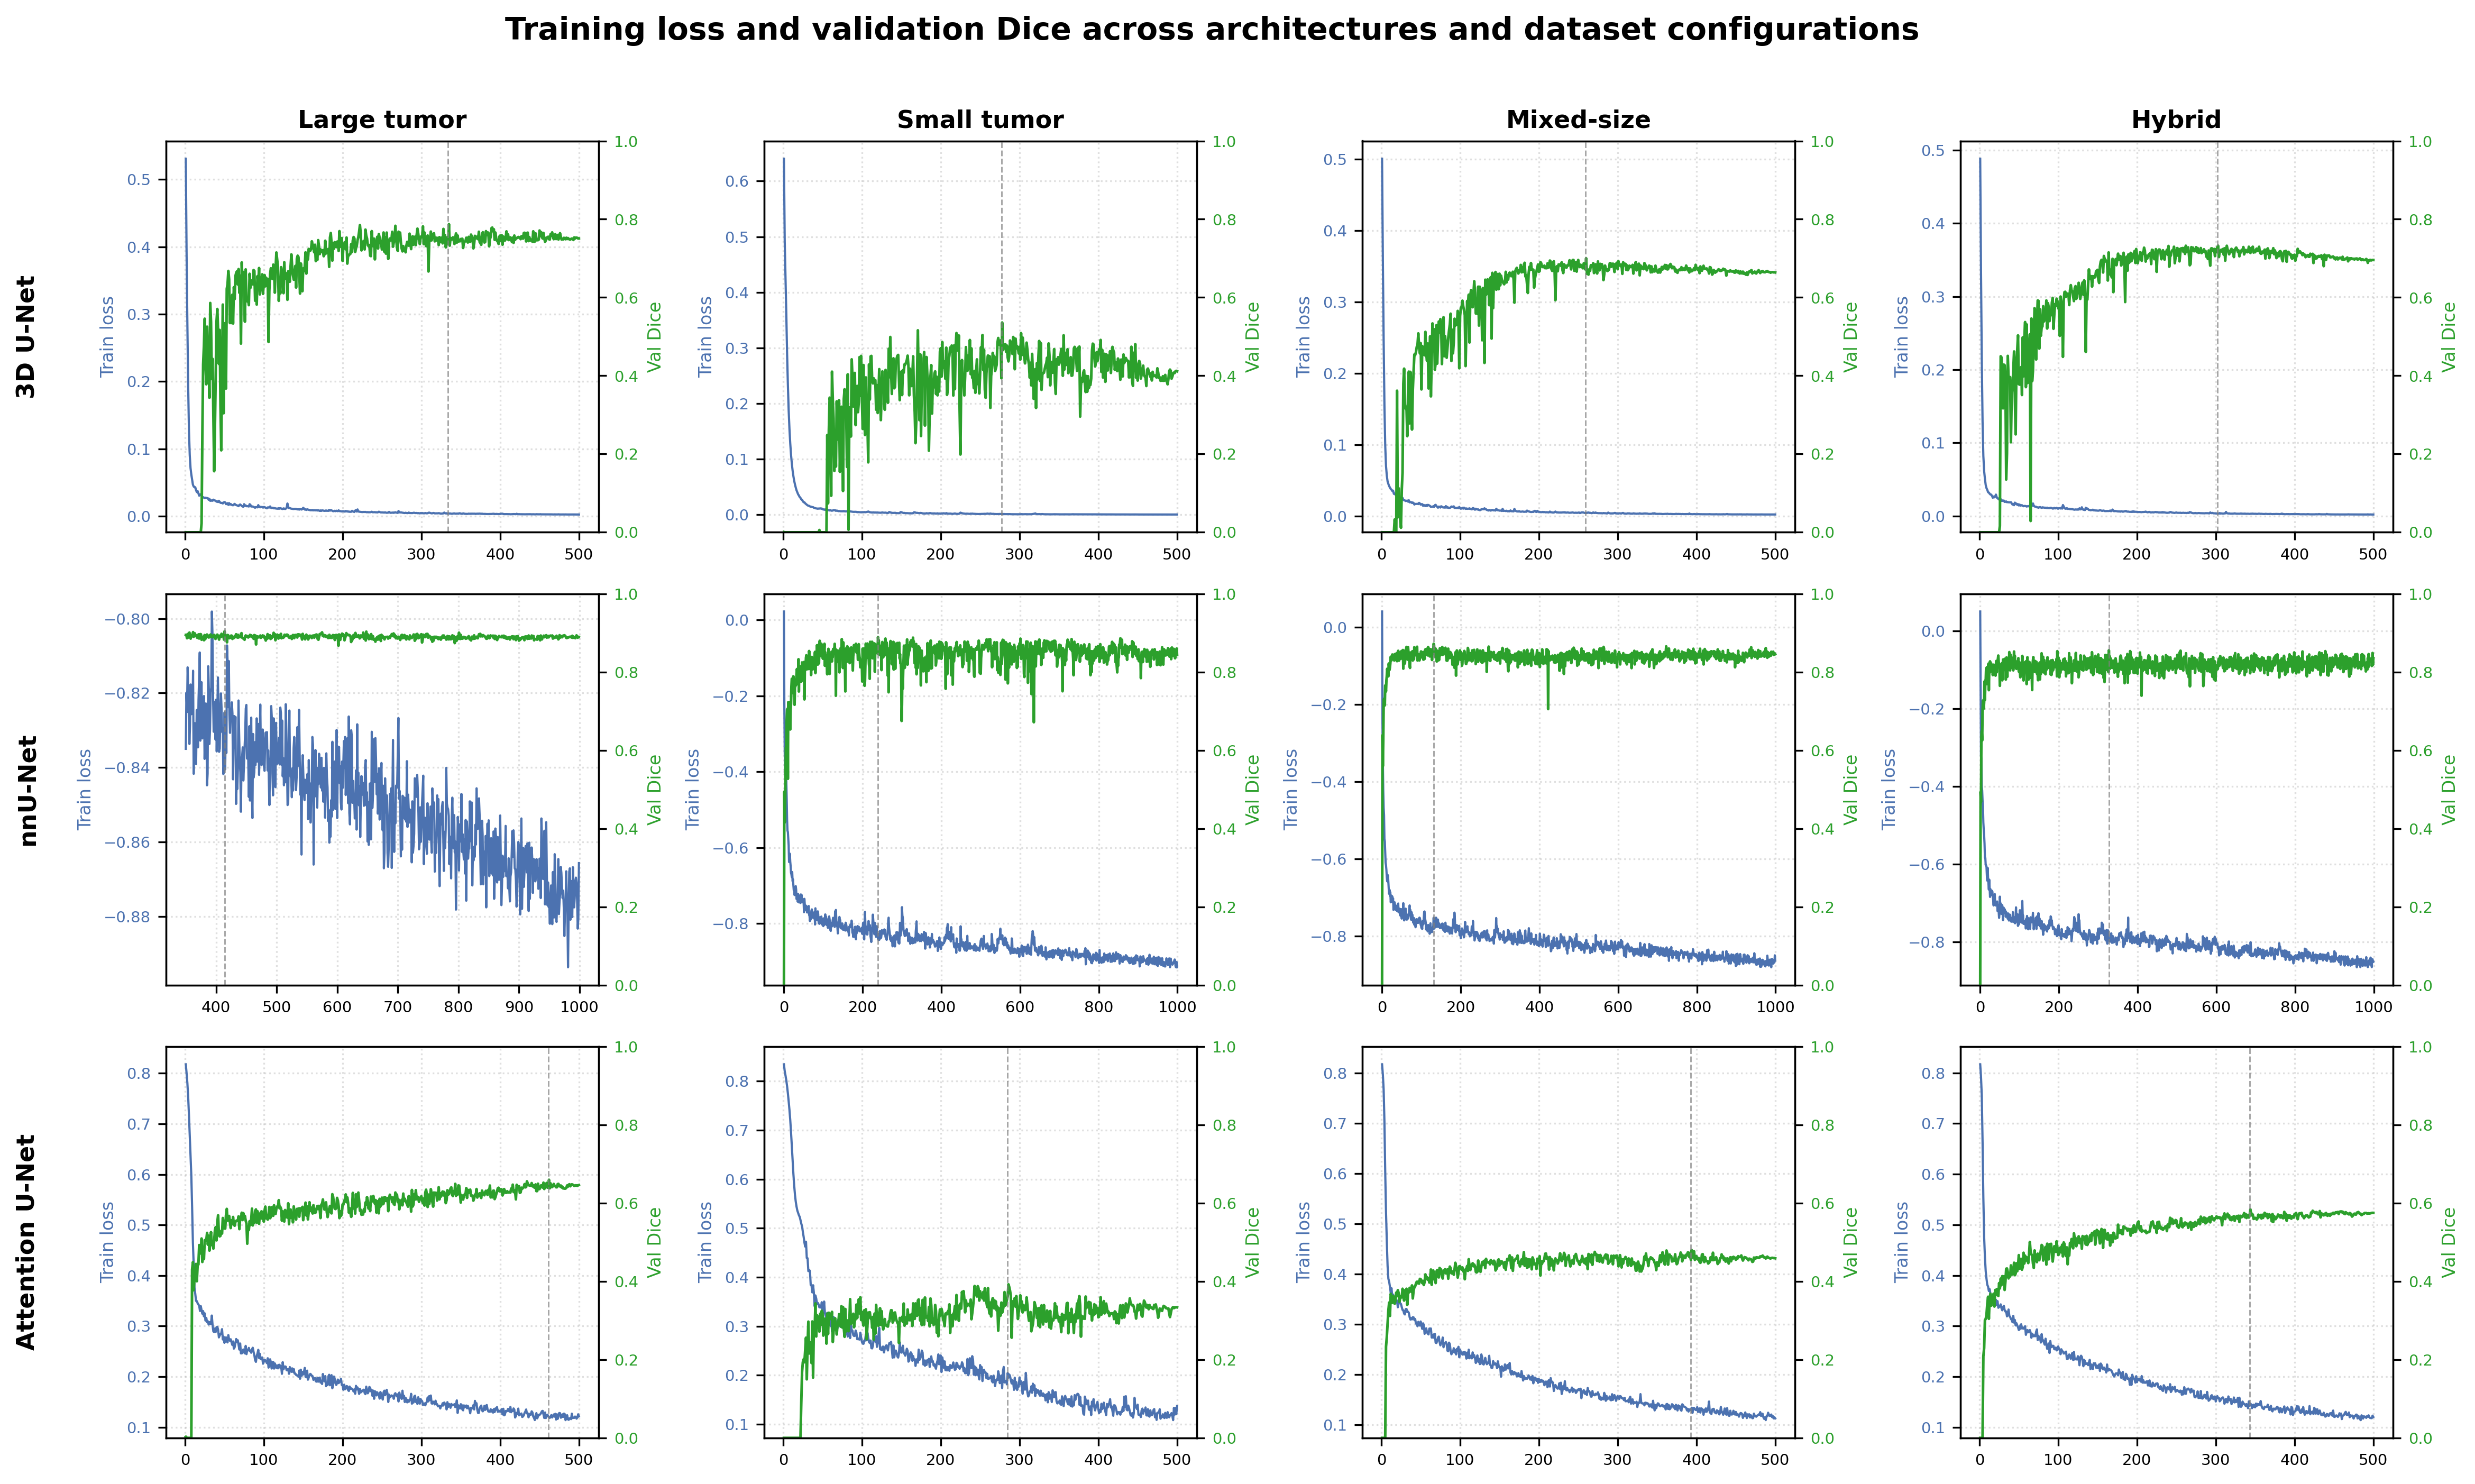
\includegraphics[width=\linewidth]{paper_assets/curves/all_arch_train_val_curves.png}
\caption{Training dynamics for all three architectures across the four dataset
configurations: training loss (blue, left axis) and validation Dice (green, right
axis); the dashed line marks the best-validation epoch. Validation Dice is shown as
the validation criterion common to all models, since per-epoch validation loss was
recorded only by nnU-Net (Figure~\ref{fig:trainval}).}
\label{fig:allarch}
\end{figure}

\subsection{Qualitative segmentation per architecture}
Figure~\ref{fig:pernet} compares the three architectures on representative clinical
test cases. For each case, rows correspond to the architectures and columns to the
input slice, ground truth, prediction, and overlay (red: ground truth; blue:
prediction; purple: overlap).

\begin{figure}[H]
\centering
\begin{subfigure}{\textwidth}\centering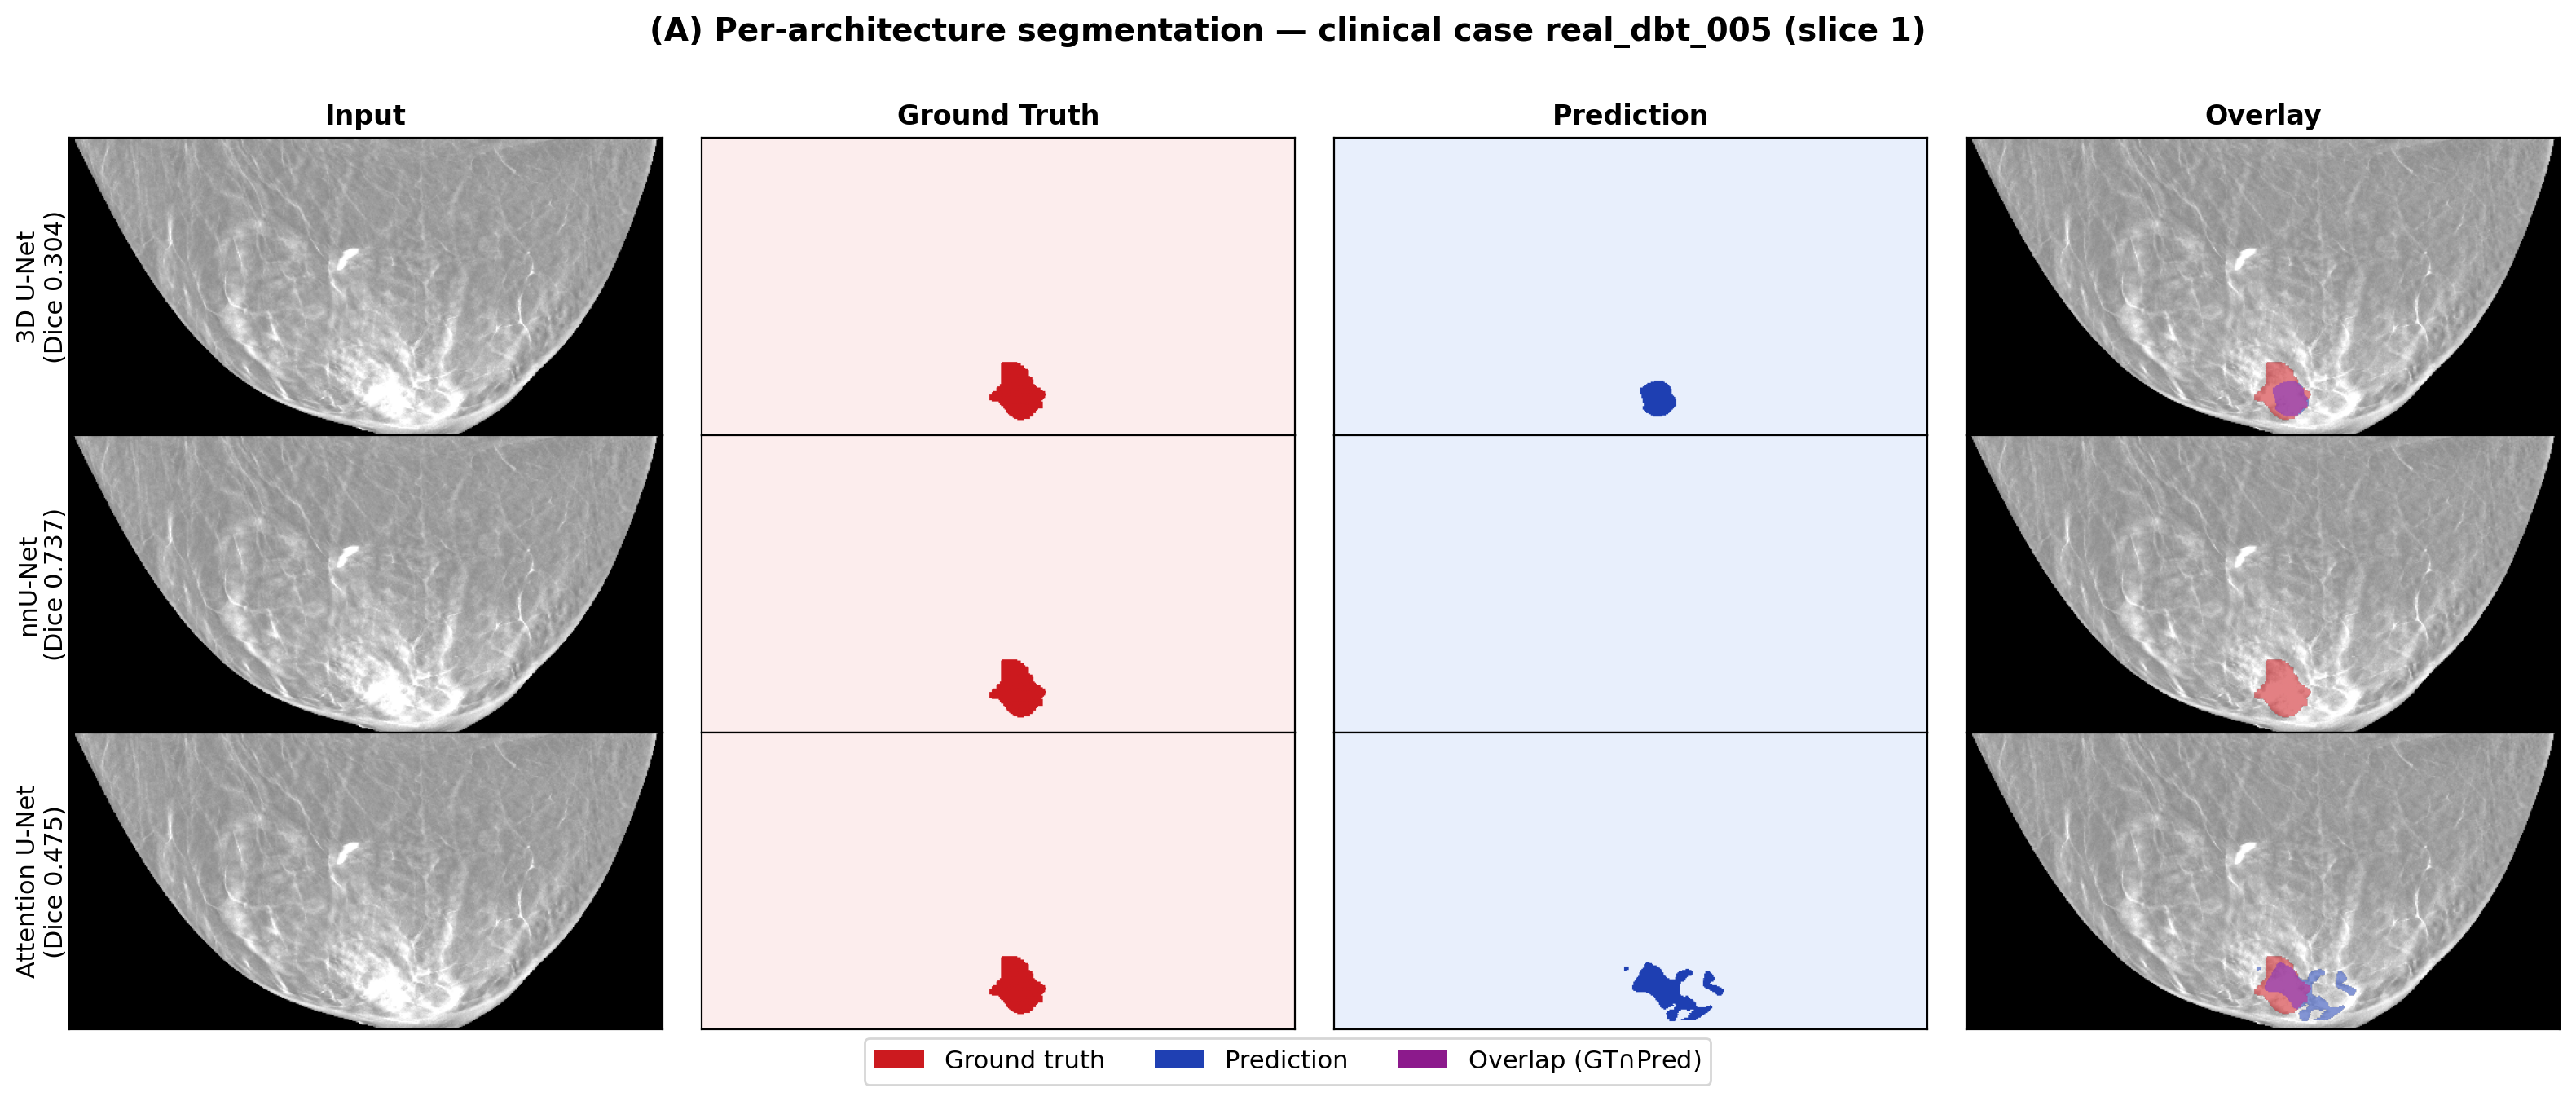
\includegraphics[width=0.82\linewidth]{paper_assets/examples/per_network_real_dbt_005.png}\caption{Clinical case with a visible lesion.}\end{subfigure}

\medskip
\begin{subfigure}{\textwidth}\centering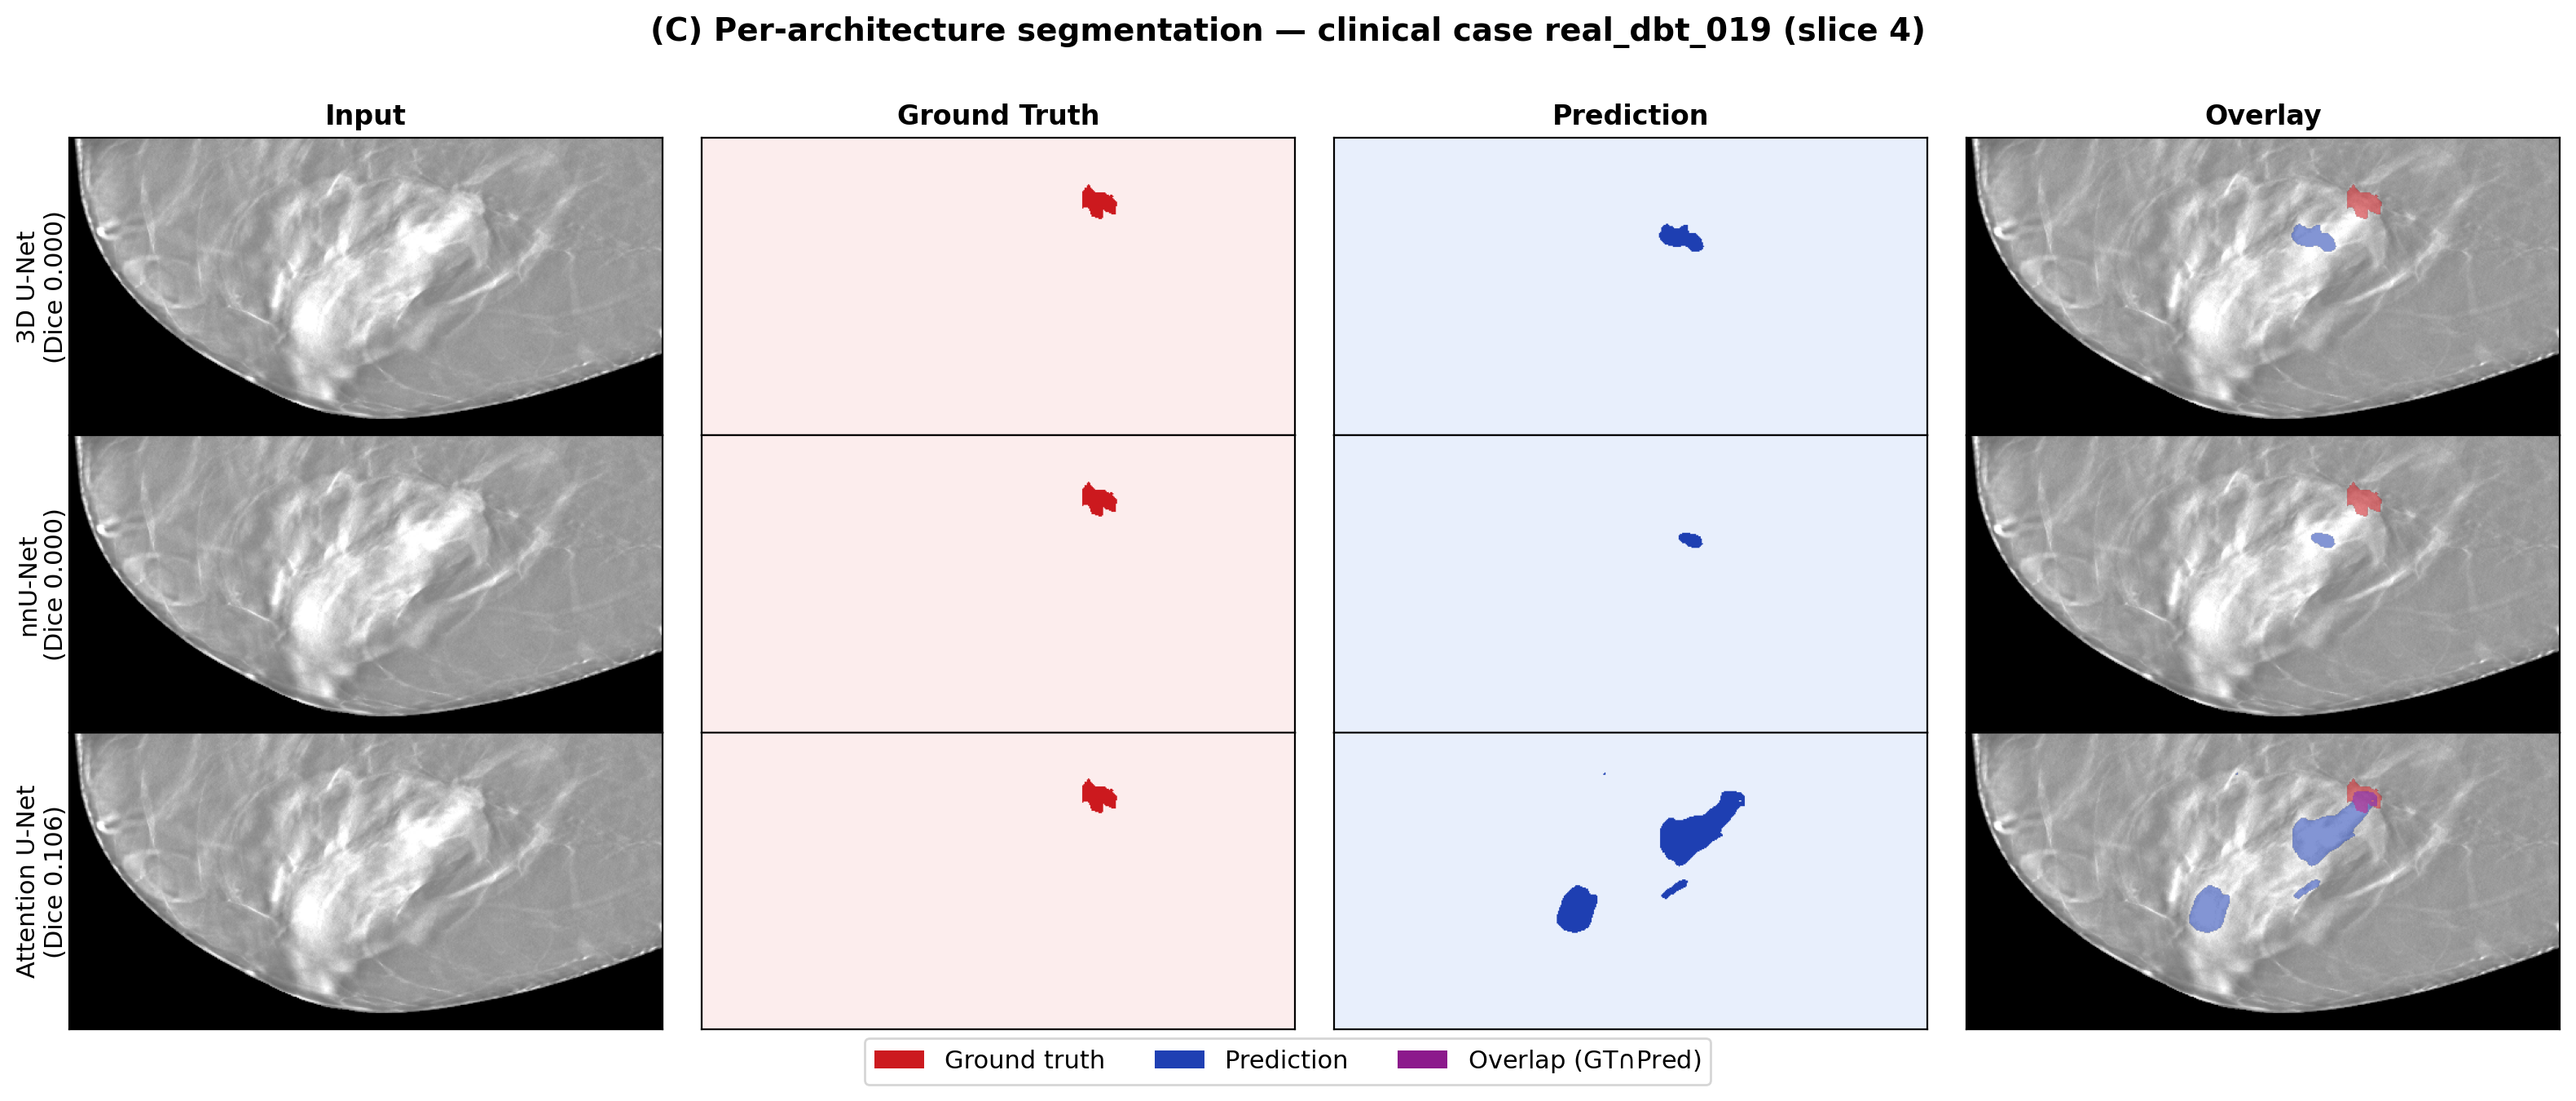
\includegraphics[width=0.82\linewidth]{paper_assets/examples/per_network_real_dbt_019.png}\caption{Low-contrast clinical lesion (hard case).}\end{subfigure}
\caption{Per-architecture qualitative segmentation on the held-out clinical test
set. Per-study Dice is annotated on each row.}
\label{fig:pernet}
\end{figure}

\subsection{Sim-to-real ensemble on clinical data}
On the held-out clinical test set, the sim-to-real ensemble outperforms every
individual fine-tuned network on Dice, IoU, and recall, and removes all empty
predictions (Table~\ref{tab:ensemble}, Figure~\ref{fig:ens}). The fine-tuning
dynamics of the nnU-Net member (Figure~\ref{fig:ftcurve}) and the qualitative
results on all ten clinical test cases (Figure~\ref{fig:ensgrid}) are also shown.

\begin{table}[H]
\centering
\caption{Clinical test performance (10 held-out cases) of the fine-tuned individual
networks and the sim-to-real ensemble (mean over cases). Best per metric in
\best{bold}.}
\label{tab:ensemble}
\small
\begin{tabular}{lcccc}
\toprule
Method & Dice & IoU & Precision & Recall \\
\midrule
nnU-Net (FT)            & 0.482 & 0.367 & \best{0.495} & 0.497 \\
Attention U-Net (FT)    & 0.372 & 0.244 & 0.291 & 0.603 \\
3D U-Net (FT)           & 0.367 & 0.249 & \best{0.496} & 0.338 \\
\textbf{Ensemble}       & \best{0.518} & \best{0.384} & 0.465 & \best{0.630} \\
\bottomrule
\end{tabular}
\end{table}

\begin{figure}[H]
\centering
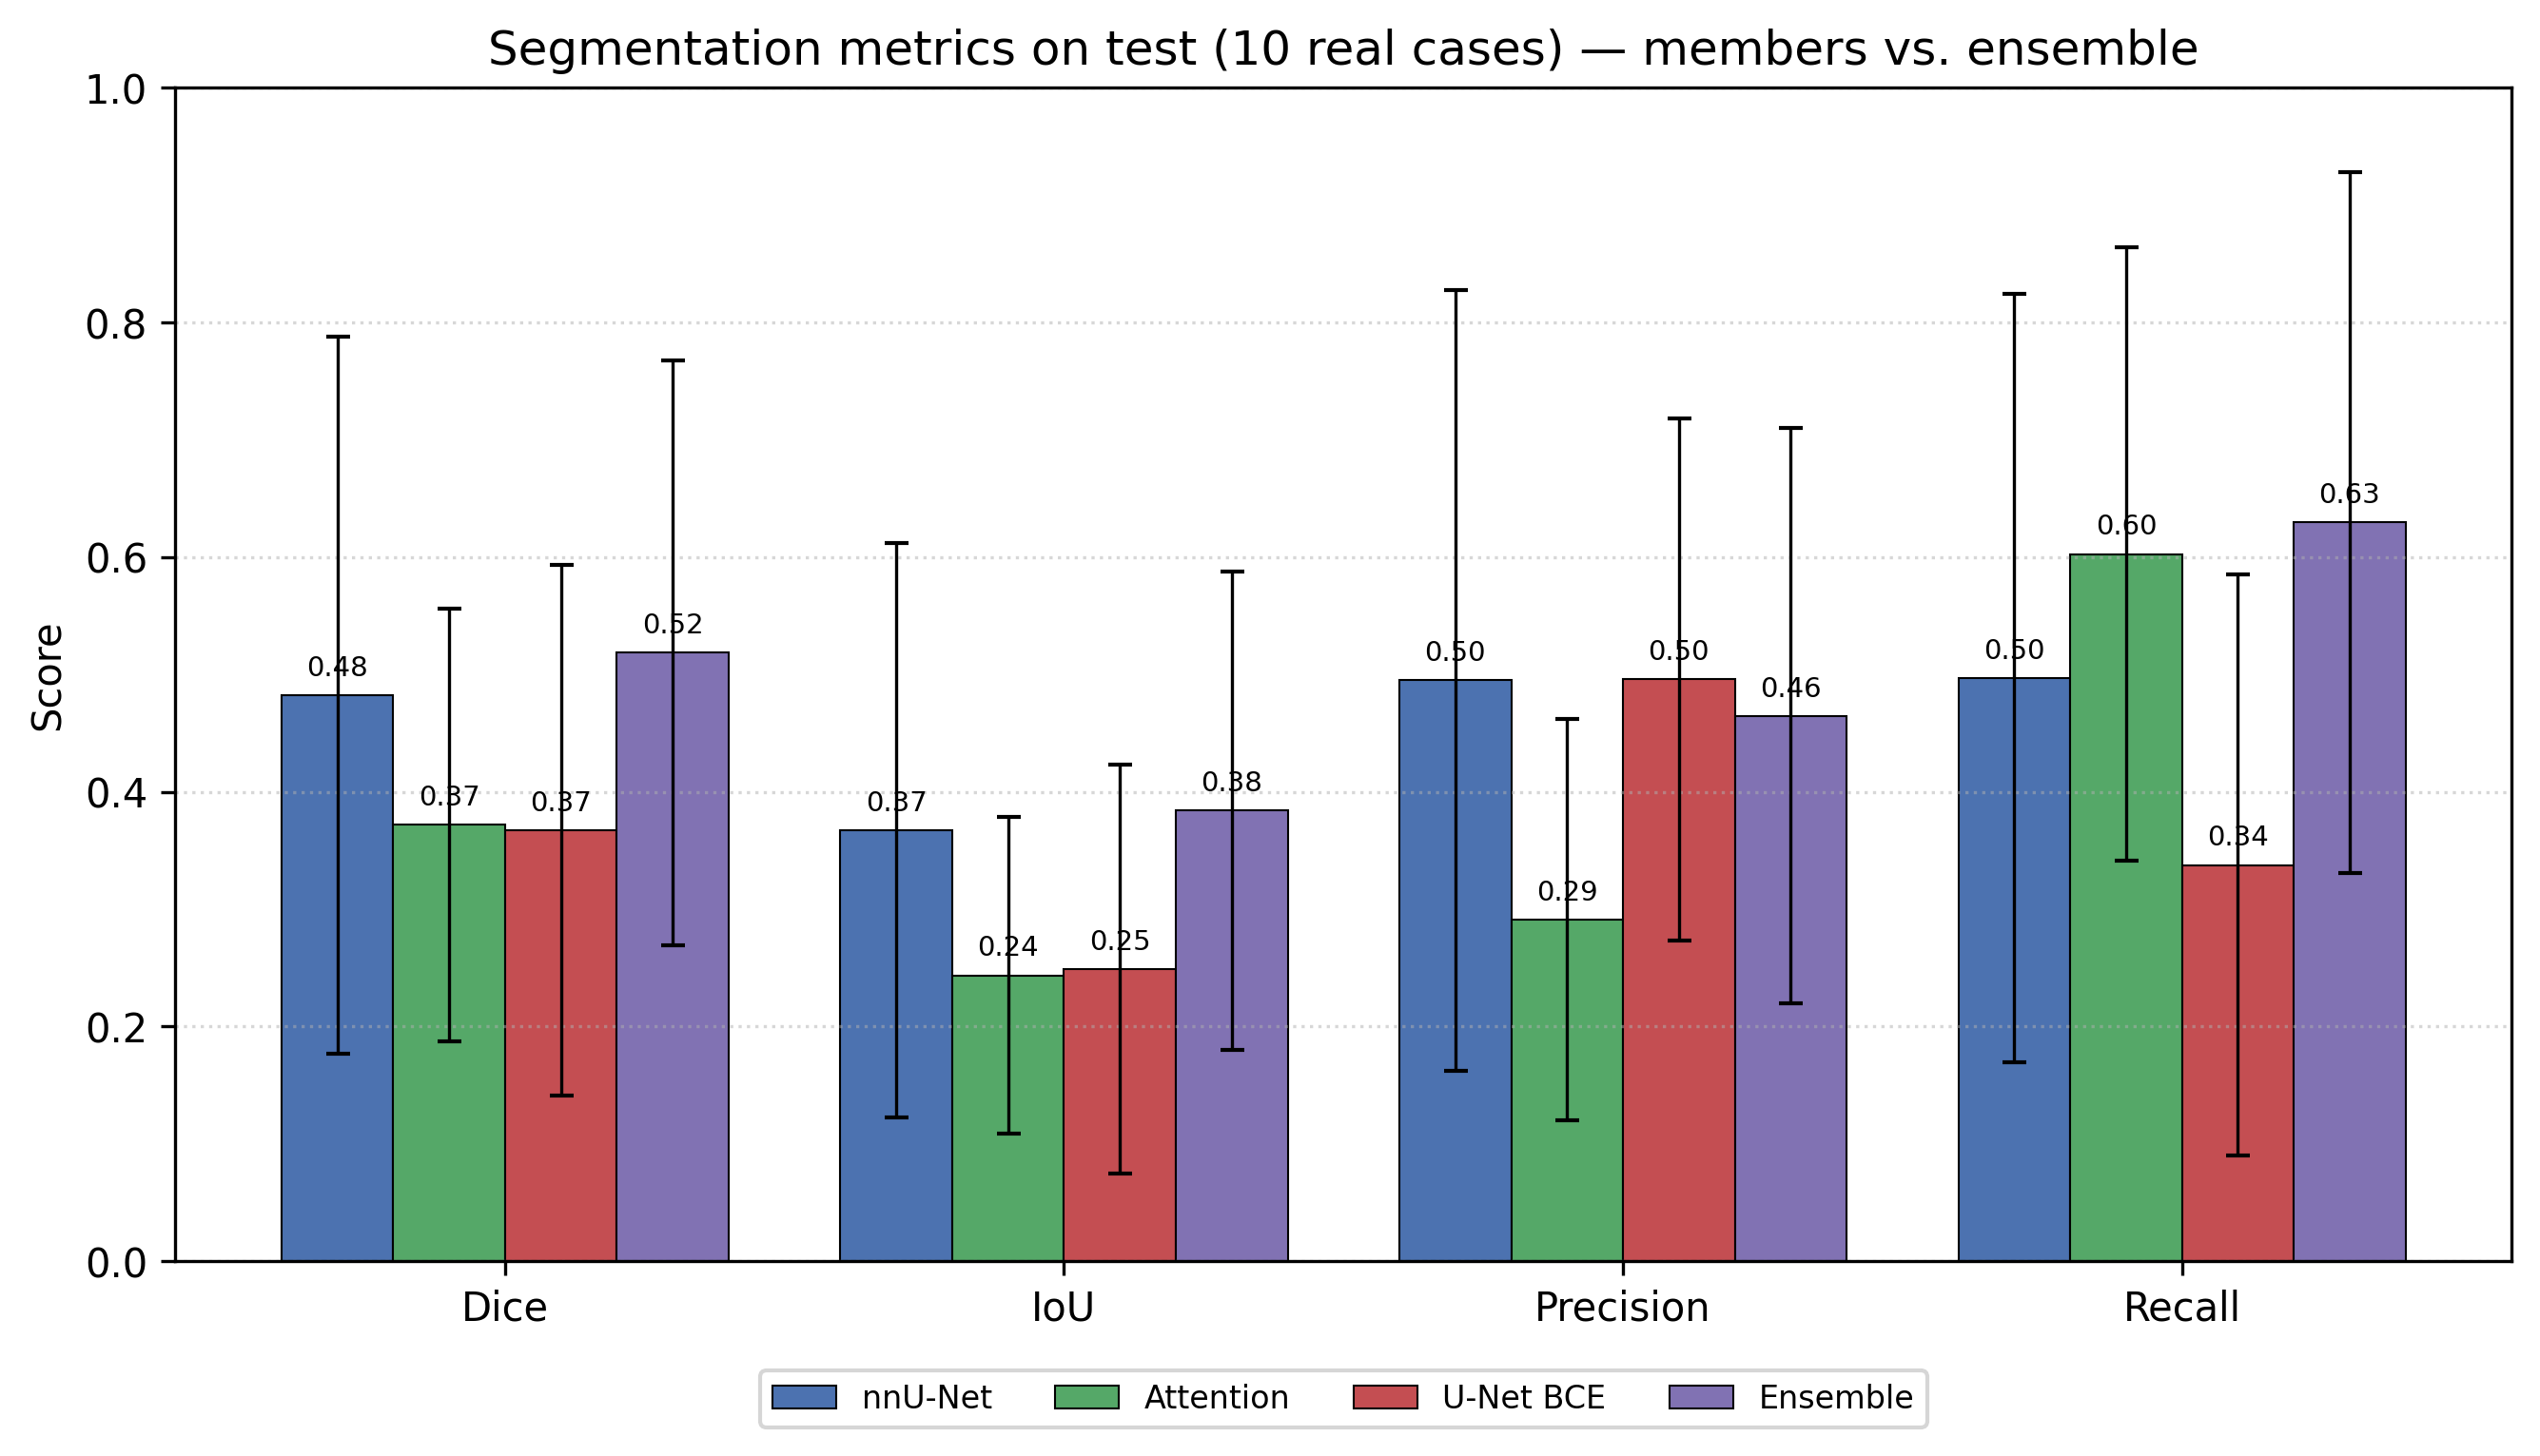
\includegraphics[width=0.78\linewidth]{paper_assets/scores/fig_scores_comparison_test.png}
\caption{Segmentation metrics (mean $\pm$ std) on the clinical test set: individual
fine-tuned networks versus the sim-to-real ensemble.}
\label{fig:ens}
\end{figure}

\begin{figure}[H]
\centering
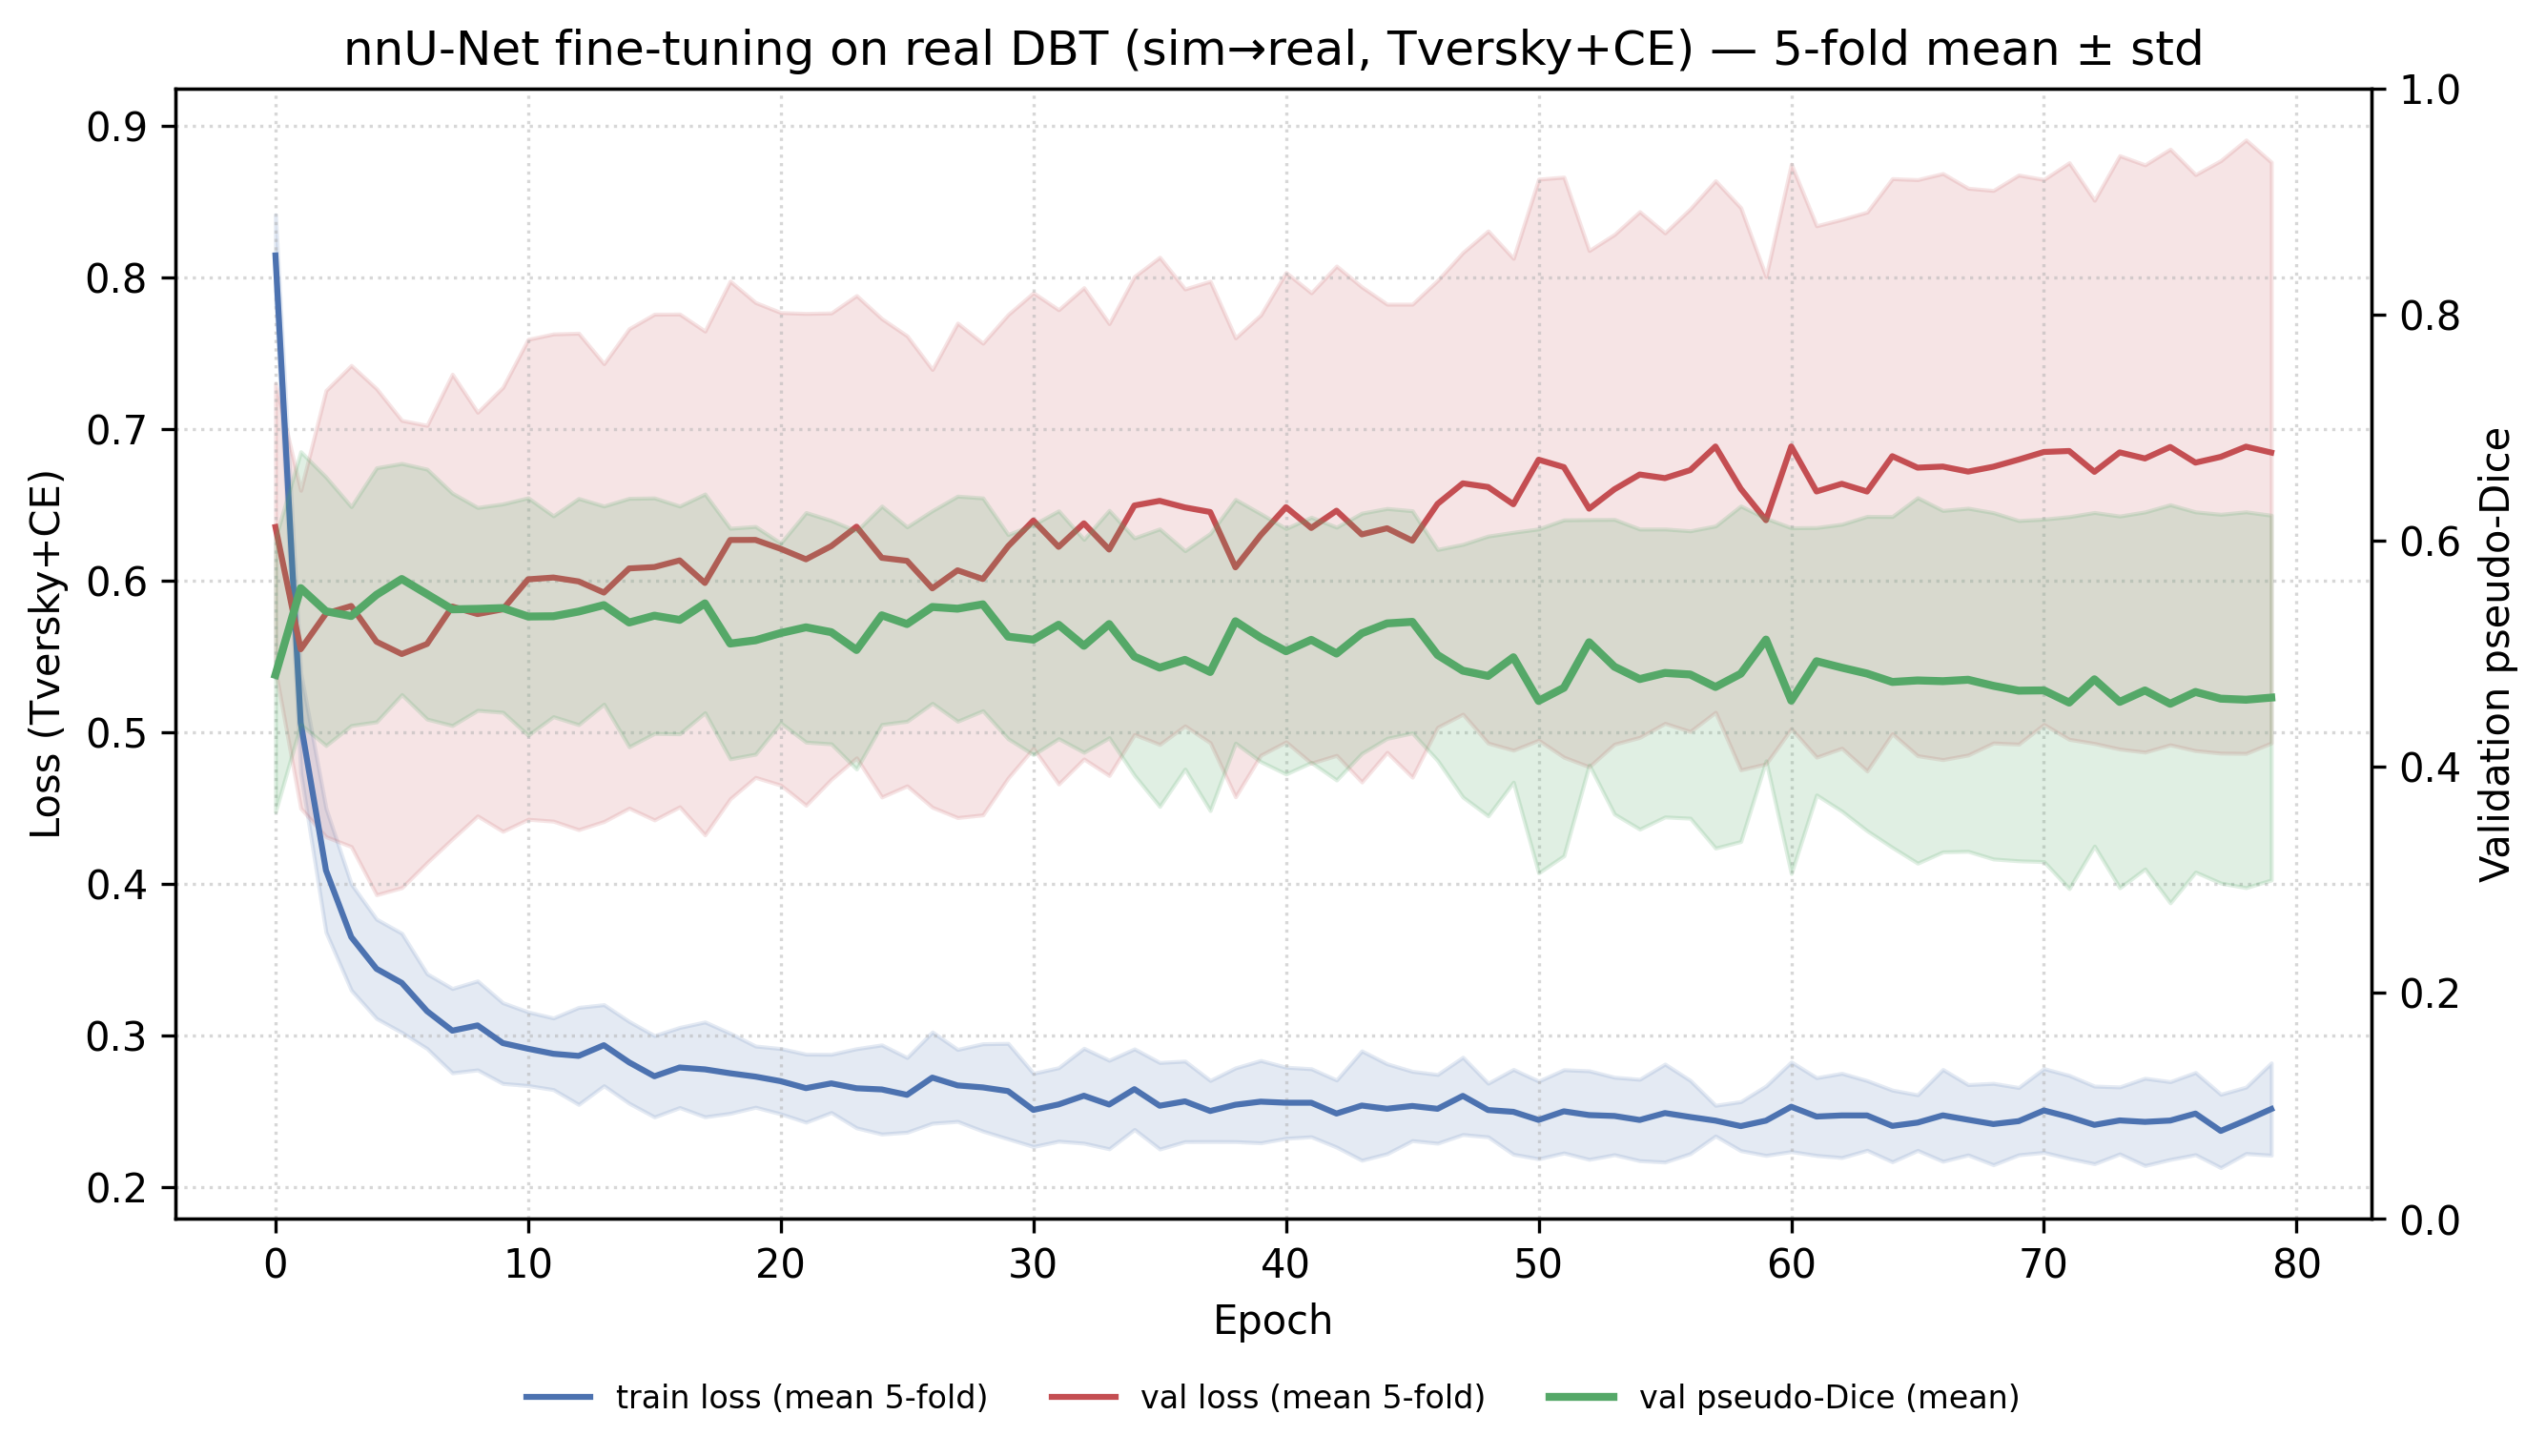
\includegraphics[width=0.72\linewidth]{paper_assets/curves/nnunet_ft_curves.png}
\caption{Fine-tuning dynamics of the nnU-Net member on the clinical development set
(sim-to-real, Tversky + CE): training loss, validation loss, and validation
pseudo-Dice (5-fold mean $\pm$ std).}
\label{fig:ftcurve}
\end{figure}

\begin{figure}[p]
\centering
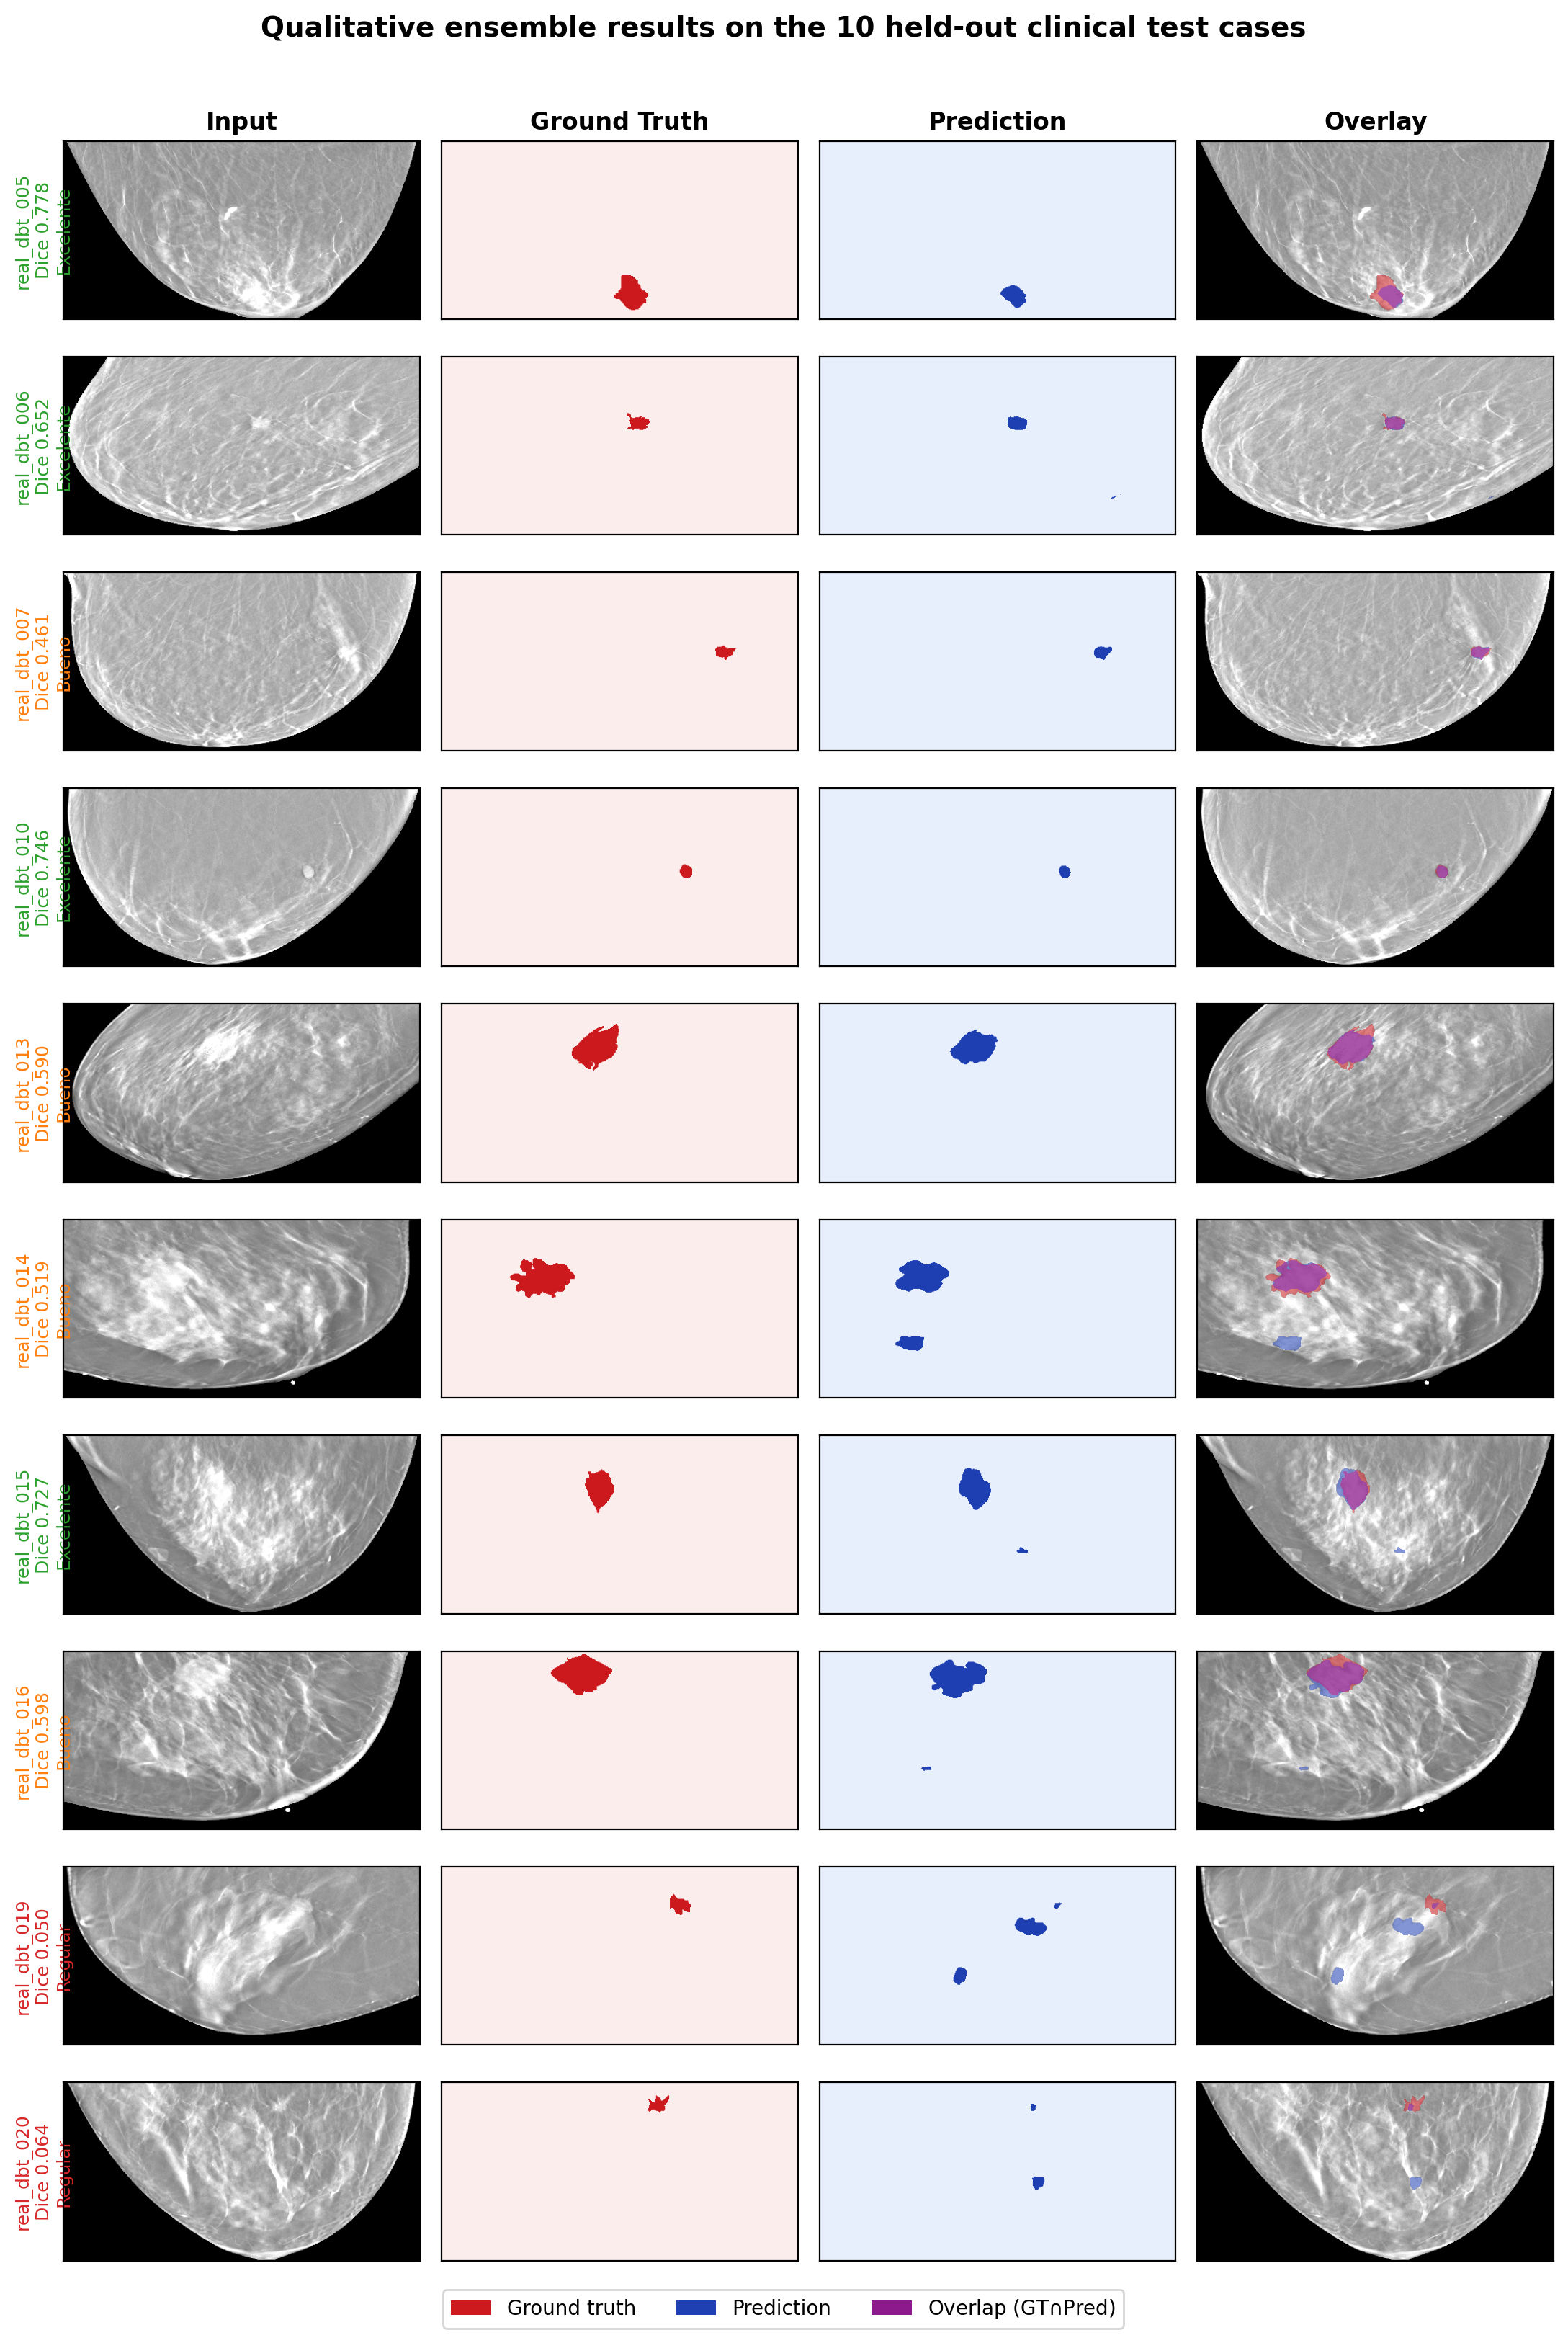
\includegraphics[height=0.92\textheight]{paper_assets/examples/examples_grid_4col_all_test.png}
\caption{Qualitative ensemble results on the ten held-out clinical test cases. Columns:
input slice, ground-truth mask, ensemble prediction, and overlay (red: ground truth;
blue: prediction; purple: overlap). Per-case Dice and quality category are annotated on
each row.}
\label{fig:ensgrid}
\end{figure}

%======================================================================
\begin{thebibliography}{99}
\small

\bibitem{bcsdbt}
Buda M, Saha A, Walsh R, Ghate S, Li N, Swiecicki A, et al.
A data set and deep learning algorithm for the detection of masses and architectural
distortions in digital breast tomosynthesis images.
\emph{JAMA Netw Open}. 2021;4(8):e2119100.

\bibitem{shia2024}
Shia WC, Kuo YH, Hsu FR, Lin J, Wu WP, Wu HK, et al.
Evaluating the margins of breast cancer tumors by using digital breast tomosynthesis
with deep learning: a preliminary assessment.
\emph{Diagnostics}. 2024;14(10):1032.

\bibitem{breastomosynth}
Alfaro-Vergara C.
BreasTomo-Synth: an in silico-generated digital breast tomosynthesis dataset for
AI-based tumor segmentation (v1). \emph{Zenodo}; 2024.

\bibitem{tsynth}
Wiedeman C, Sarmakeeva A, Sizikova E, Filienko D, Lago MA, Delfino JG, et al.
T-SYNTH: a knowledge-based dataset of synthetic breast images.
\emph{arXiv}:2507.04038; 2025.

\bibitem{alfaro2025}
Alfaro Vergara C, Araya Caro N, Mery Quiroz D, Prieto Vasquez C.
In silico digital breast tomosynthesis dataset for the comparative analysis of deep
learning models in tumor segmentation.
\emph{J Imaging Inform Med}. 2025.

\bibitem{cicek2016}
{\c{C}}i{\c{c}}ek {\"O}, Abdulkadir A, Lienkamp SS, Brox T, Ronneberger O.
3D U-Net: learning dense volumetric segmentation from sparse annotation.
\emph{MICCAI}; 2016. Springer.

\bibitem{isensee2021}
Isensee F, Jaeger PF, Kohl SAA, Petersen J, Maier-Hein KH.
nnU-Net: a self-configuring method for deep learning-based biomedical image
segmentation. \emph{Nature Methods}. 2021;18(2):203--211.

\bibitem{isensee2018}
Isensee F, Petersen J, Klein A, Zimmerer D, Jaeger PF, Kohl S, et al.
nnU-Net: self-adapting framework for U-Net-based medical image segmentation.
\emph{arXiv}:1809.10486; 2018.

\bibitem{oktay2018}
Oktay O, Schlemper J, Folgoc LL, Lee M, Heinrich M, Misawa K, et al.
Attention U-Net: learning where to look for the pancreas.
\emph{arXiv}:1804.03999; 2018.

\bibitem{victre_pipeline}
VICTRE Automatic Pipeline. Available from:
\url{https://github.com/DIDSR/VICTRE_PIPELINE}.

\bibitem{badano2018}
Badano A, Graff CG, Badal A, Sharma D, Zeng R, Samuelson FW, et al.
Evaluation of digital breast tomosynthesis as replacement of full-field digital
mammography using an in silico imaging trial.
\emph{JAMA Netw Open}. 2018;1(7):e185474.

\bibitem{fiji}
Schindelin J, Arganda-Carreras I, Frise E, Kaynig V, Longair M, Pietzsch T, et al.
Fiji: an open-source platform for biological-image analysis.
\emph{Nature Methods}. 2012;9(7):676--682.

\bibitem{loshchilov2017}
Loshchilov I, Hutter F.
Decoupled weight decay regularization.
\emph{arXiv}:1711.05101; 2017.

\bibitem{micikevicius2017}
Micikevicius P, Narang S, Alben J, Diamos GF, Elsen E, Garc{\'i}a D, et al.
Mixed precision training. \emph{arXiv}:1710.03740; 2017.

\end{thebibliography}

\end{document}
